\documentclass[twoside]{book}

% Packages required by doxygen
\usepackage{calc}
\usepackage{doxygen}
\usepackage{graphicx}
\usepackage[utf8]{inputenc}
\usepackage{makeidx}
\usepackage{multicol}
\usepackage{multirow}
\usepackage{textcomp}
\usepackage[table]{xcolor}

% Font selection
\usepackage[T1]{fontenc}
\usepackage{mathptmx}
\usepackage[scaled=.90]{helvet}
\usepackage{courier}
\usepackage{amssymb}
\usepackage{sectsty}
\renewcommand{\familydefault}{\sfdefault}
\allsectionsfont{%
  \fontseries{bc}\selectfont%
  \color{darkgray}%
}
\renewcommand{\DoxyLabelFont}{%
  \fontseries{bc}\selectfont%
  \color{darkgray}%
}

% Page & text layout
\usepackage{geometry}
\geometry{%
  a4paper,%
  top=2.5cm,%
  bottom=2.5cm,%
  left=2.5cm,%
  right=2.5cm%
}
\tolerance=750
\hfuzz=15pt
\hbadness=750
\setlength{\emergencystretch}{15pt}
\setlength{\parindent}{0cm}
\setlength{\parskip}{0.2cm}
\makeatletter
\renewcommand{\paragraph}{%
  \@startsection{paragraph}{4}{0ex}{-1.0ex}{1.0ex}{%
    \normalfont\normalsize\bfseries\SS@parafont%
  }%
}
\renewcommand{\subparagraph}{%
  \@startsection{subparagraph}{5}{0ex}{-1.0ex}{1.0ex}{%
    \normalfont\normalsize\bfseries\SS@subparafont%
  }%
}
\makeatother

% Headers & footers
\usepackage{fancyhdr}
\pagestyle{fancyplain}
\fancyhead[LE]{\fancyplain{}{\bfseries\thepage}}
\fancyhead[CE]{\fancyplain{}{}}
\fancyhead[RE]{\fancyplain{}{\bfseries\leftmark}}
\fancyhead[LO]{\fancyplain{}{\bfseries\rightmark}}
\fancyhead[CO]{\fancyplain{}{}}
\fancyhead[RO]{\fancyplain{}{\bfseries\thepage}}
\fancyfoot[LE]{\fancyplain{}{}}
\fancyfoot[CE]{\fancyplain{}{}}
\fancyfoot[RE]{\fancyplain{}{\bfseries\scriptsize Generated on Sat Jun 3 2017 22\-:06\-:01 for S\-Q\-Lite\-X\-X by Doxygen }}
\fancyfoot[LO]{\fancyplain{}{\bfseries\scriptsize Generated on Sat Jun 3 2017 22\-:06\-:01 for S\-Q\-Lite\-X\-X by Doxygen }}
\fancyfoot[CO]{\fancyplain{}{}}
\fancyfoot[RO]{\fancyplain{}{}}
\renewcommand{\footrulewidth}{0.4pt}
\renewcommand{\chaptermark}[1]{%
  \markboth{#1}{}%
}
\renewcommand{\sectionmark}[1]{%
  \markright{\thesection\ #1}%
}

% Indices & bibliography
\usepackage{natbib}
\usepackage[titles]{tocloft}
\setcounter{tocdepth}{3}
\setcounter{secnumdepth}{5}
\makeindex

% Hyperlinks (required, but should be loaded last)
\usepackage{ifpdf}
\ifpdf
  \usepackage[pdftex,pagebackref=true]{hyperref}
\else
  \usepackage[ps2pdf,pagebackref=true]{hyperref}
\fi
\hypersetup{%
  colorlinks=true,%
  linkcolor=blue,%
  citecolor=blue,%
  unicode%
}

% Custom commands
\newcommand{\clearemptydoublepage}{%
  \newpage{\pagestyle{empty}\cleardoublepage}%
}


%===== C O N T E N T S =====

\begin{document}

% Titlepage & ToC
\hypersetup{pageanchor=false}
\pagenumbering{roman}
\begin{titlepage}
\vspace*{7cm}
\begin{center}%
{\Large S\-Q\-Lite\-X\-X \\[1ex]\large 0.\-1.\-0 }\\
\vspace*{1cm}
{\large Generated by Doxygen 1.8.6}\\
\vspace*{0.5cm}
{\small Sat Jun 3 2017 22:06:01}\\
\end{center}
\end{titlepage}
\clearemptydoublepage
\tableofcontents
\clearemptydoublepage
\pagenumbering{arabic}
\hypersetup{pageanchor=true}

%--- Begin generated contents ---
\chapter{Main Page}
\label{index}\hypertarget{index}{}\href{https://github.com/maxxboehme/SQLiteXX/blob/master/LICENSE.txt}{\tt !\mbox{[}License\mbox{]}(https\-://img.\-shields.\-io/badge/license-\/\-M\-I\-T-\/blue.\-svg)} \href{https://travis-ci.org/maxxboehme/SQLiteXX}{\tt !\mbox{[}Travis C\-I Linux/\-Mac Build Status\mbox{]}(https\-://travis-\/ci.\-org/maxxboehme/\-S\-Q\-Lite\-X\-X.\-svg?branch=master)} \href{https://ci.appveyor.com/project/maxxboehme/sqlitexx/branch/master}{\tt !\mbox{[}App\-Veyor Windows Build status\mbox{]}(https\-://ci.\-appveyor.\-com/api/projects/status/wkrlgfv2p5mm5cgg/branch/master?svg=true)} \href{https://coveralls.io/github/maxxboehme/SQLiteXX}{\tt !\mbox{[}Coverage Status\mbox{]}(https\-://coveralls.\-io/repos/github/maxxboehme/\-S\-Q\-Lite\-X\-X/badge.\-svg)}

\subsection*{What is S\-Q\-Lite\-X\-X}

A C++ wrapper for sqlite3 that uses features in C++14.

\subsection*{How to use it}

The following links will direct you to helpful documents on how to use S\-Q\-Lite\-X\-X.


\begin{DoxyItemize}
\item https\-://github.com/maxxboehme/\-S\-Q\-Lite\-X\-X/blob/master/docs/tutorial.\-md \char`\"{}\-Tutorial\char`\"{} -\/ Getting Started
\item \href{https://maxxboehme.github.io/SQLiteXX/doxygen/html}{\tt Doxygen} -\/ Documentation for the A\-P\-I
\item https\-://github.com/maxxboehme/\-S\-Q\-Lite\-X\-X/blob/master/docs/\-Read\-Me.\-md \char`\"{}\-Reference\char`\"{} -\/ all the details
\end{DoxyItemize}

\subsection*{How to build it}

You will need a compiler that supports C++14. The Travis-\/\-C\-I Y\-A\-M\-L file shows some of the supported compilers.

\subsection*{More}


\begin{DoxyItemize}
\item Issues and bugs can be raised on the \href{https://github.com/maxxboehme/SQLiteXX/issues}{\tt Issue tracker on Github} 
\end{DoxyItemize}
\chapter{Hierarchical Index}
\section{Class Hierarchy}
This inheritance list is sorted roughly, but not completely, alphabetically\-:\begin{DoxyCompactList}
\item \contentsline{section}{sqlite\-:\-:backup}{\pageref{a00001}}{}
\item \contentsline{section}{sqlite\-:\-:blob}{\pageref{a00002}}{}
\item \contentsline{section}{sqlite\-:\-:dbconnection}{\pageref{a00004}}{}
\item \contentsline{section}{sqlite\-:\-:exception}{\pageref{a00006}}{}
\begin{DoxyCompactList}
\item \contentsline{section}{sqlite\-:\-:busy\-\_\-exception}{\pageref{a00003}}{}
\end{DoxyCompactList}
\item \contentsline{section}{sqlite\-:\-:mutex}{\pageref{a00009}}{}
\item \contentsline{section}{sqlite\-:\-:reader$<$ T $>$}{\pageref{a00010}}{}
\item \contentsline{section}{sqlite\-:\-:reader$<$ row $>$}{\pageref{a00010}}{}
\begin{DoxyCompactList}
\item \contentsline{section}{sqlite\-:\-:row}{\pageref{a00011}}{}
\end{DoxyCompactList}
\item \contentsline{section}{sqlite\-:\-:reader$<$ statement $>$}{\pageref{a00010}}{}
\begin{DoxyCompactList}
\item \contentsline{section}{sqlite\-:\-:statement}{\pageref{a00013}}{}
\end{DoxyCompactList}
\item \contentsline{section}{sqlite\-:\-:row\-\_\-iterator}{\pageref{a00012}}{}
\item \contentsline{section}{sqlite\-:\-:transaction}{\pageref{a00014}}{}
\begin{DoxyCompactList}
\item \contentsline{section}{sqlite\-:\-:deferred\-\_\-transaction}{\pageref{a00005}}{}
\item \contentsline{section}{sqlite\-:\-:exclusive\-\_\-transaction}{\pageref{a00007}}{}
\item \contentsline{section}{sqlite\-:\-:immediate\-\_\-transaction}{\pageref{a00008}}{}
\end{DoxyCompactList}
\item \contentsline{section}{sqlite\-:\-:value}{\pageref{a00015}}{}
\end{DoxyCompactList}

\chapter{Class Index}
\section{Class List}
Here are the classes, structs, unions and interfaces with brief descriptions\-:\begin{DoxyCompactList}
\item\contentsline{section}{\hyperlink{a00001}{sqlite\-::backup} \\*Used to aid in the process of backing up a database }{\pageref{a00001}}{}
\item\contentsline{section}{\hyperlink{a00002}{sqlite\-::blob} \\*A \char`\"{}\-Binary Large O\-Bject\char`\"{} }{\pageref{a00002}}{}
\item\contentsline{section}{\hyperlink{a00003}{sqlite\-::busy\-\_\-exception} \\*Encapsulation of the S\-Q\-L\-I\-T\-E\-\_\-\-B\-U\-S\-Y error code derived from S\-Q\-Lite\-::\-Exception }{\pageref{a00003}}{}
\item\contentsline{section}{\hyperlink{a00004}{sqlite\-::dbconnection} \\*Class that represents a connection to a database }{\pageref{a00004}}{}
\item\contentsline{section}{\hyperlink{a00005}{sqlite\-::deferred\-\_\-transaction} \\*R\-A\-I\-I encapsulation of the \hyperlink{a00038}{S\-Q\-Lite} deferred transaction }{\pageref{a00005}}{}
\item\contentsline{section}{\hyperlink{a00006}{sqlite\-::exception} \\*Encapsulation of the error code and message from S\-Q\-Lite3, based on std\-::runtime\-\_\-error }{\pageref{a00006}}{}
\item\contentsline{section}{\hyperlink{a00007}{sqlite\-::exclusive\-\_\-transaction} \\*R\-A\-I\-I encapsulation of the \hyperlink{a00038}{S\-Q\-Lite} exclusive transaction }{\pageref{a00007}}{}
\item\contentsline{section}{\hyperlink{a00008}{sqlite\-::immediate\-\_\-transaction} \\*R\-A\-I\-I encapsulation of the \hyperlink{a00038}{S\-Q\-Lite} immediate transaction }{\pageref{a00008}}{}
\item\contentsline{section}{\hyperlink{a00009}{sqlite\-::mutex} \\*Helps with serializing access to a database connection }{\pageref{a00009}}{}
\item\contentsline{section}{\hyperlink{a00010}{sqlite\-::reader$<$ T $>$} \\*Base class used to help with reading \char`\"{}sqlite3\-\_\-stmt\char`\"{} information }{\pageref{a00010}}{}
\item\contentsline{section}{\hyperlink{a00011}{sqlite\-::row} \\*Represents a returned row when stepping through a \char`\"{}\-S\-E\-L\-E\-C\-T\char`\"{} statement }{\pageref{a00011}}{}
\item\contentsline{section}{\hyperlink{a00012}{sqlite\-::row\-\_\-iterator} \\*Helps when iterating over rows in a \char`\"{}\-S\-E\-L\-E\-C\-T\char`\"{} statement }{\pageref{a00012}}{}
\item\contentsline{section}{\hyperlink{a00013}{sqlite\-::statement} \\*Represents a single S\-Q\-L statement that has been compiled into binary form and is ready to be evaluated, aka \char`\"{}sqlite3\-\_\-stmt\char`\"{} }{\pageref{a00013}}{}
\item\contentsline{section}{\hyperlink{a00014}{sqlite\-::transaction} \\*R\-A\-I\-I encapsulation of the \hyperlink{a00038}{S\-Q\-Lite} Transactions }{\pageref{a00014}}{}
\item\contentsline{section}{\hyperlink{a00015}{sqlite\-::value} \\*A \hyperlink{a00038}{S\-Q\-Lite} dynamically typed value object, aka \char`\"{}sqlite3\-\_\-value\char`\"{} }{\pageref{a00015}}{}
\end{DoxyCompactList}

\chapter{Class Documentation}
\hypertarget{a00001}{\section{S\-Q\-Lite\-:\-:Busy\-Exception Class Reference}
\label{a00001}\index{S\-Q\-Lite\-::\-Busy\-Exception@{S\-Q\-Lite\-::\-Busy\-Exception}}
}


Encapsulation of the S\-Q\-L\-I\-T\-E\-\_\-\-B\-U\-S\-Y error code derived from \hyperlink{a00003}{S\-Q\-Lite\-::\-Exception}.  




{\ttfamily \#include $<$Exception.\-h$>$}

Inheritance diagram for S\-Q\-Lite\-:\-:Busy\-Exception\-:\begin{figure}[H]
\begin{center}
\leavevmode
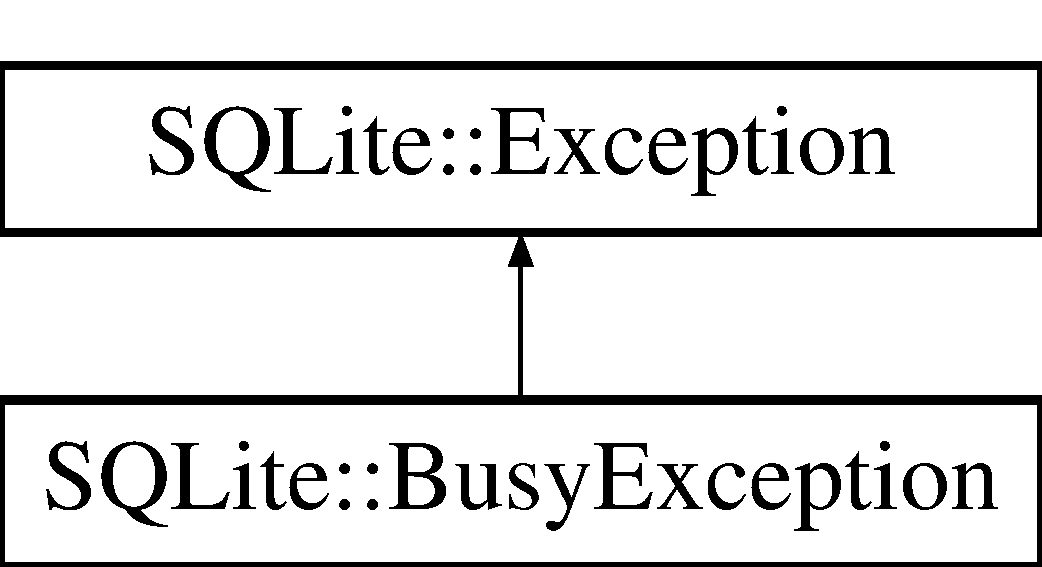
\includegraphics[height=2.000000cm]{a00001}
\end{center}
\end{figure}


\subsection{Detailed Description}
Encapsulation of the S\-Q\-L\-I\-T\-E\-\_\-\-B\-U\-S\-Y error code derived from \hyperlink{a00003}{S\-Q\-Lite\-::\-Exception}. 



Definition at line 33 of file Exception.\-h.



The documentation for this class was generated from the following file\-:\begin{DoxyCompactItemize}
\item 
src/Exception.\-h\end{DoxyCompactItemize}

\hypertarget{a00002}{\section{sqlite\-:\-:blob Class Reference}
\label{a00002}\index{sqlite\-::blob@{sqlite\-::blob}}
}


A \char`\"{}\-Binary Large O\-Bject\char`\"{}.  




{\ttfamily \#include $<$Blob.\-h$>$}

\subsection*{Public Member Functions}
\begin{DoxyCompactItemize}
\item 
\hyperlink{a00002_ad3d7146a3081de7c96a37b9641f83dd6}{blob} (const void $\ast$\hyperlink{a00002_ad9fc3eb820ef6fa64a4a03224b9dc3de}{data}, const size\-\_\-t \hyperlink{a00002_a28b69b40596ded278607604396b86c97}{size})
\begin{DoxyCompactList}\small\item\em Constructs a blob object with contents of data. \end{DoxyCompactList}\item 
\hyperlink{a00002_a1f1bca1ecf4615c4948f3af74814abde}{blob} (const \hyperlink{a00002}{blob} \&other)
\begin{DoxyCompactList}\small\item\em Copy constructor. \end{DoxyCompactList}\item 
\hyperlink{a00002_a78501ec4704d95d590457eacc63f39b6}{blob} (\hyperlink{a00002}{blob} \&\&other)
\begin{DoxyCompactList}\small\item\em Move constructor. \end{DoxyCompactList}\item 
\hyperlink{a00002}{blob} \& \hyperlink{a00002_a1962255cded865181174a67351d58fb8}{operator=} (const \hyperlink{a00002}{blob} \&other)
\begin{DoxyCompactList}\small\item\em Copy assignment operator. \end{DoxyCompactList}\item 
\hyperlink{a00002}{blob} \& \hyperlink{a00002_a93a890b30c970d76fc51ad7ed4bb36c1}{operator=} (\hyperlink{a00002}{blob} \&\&other)
\begin{DoxyCompactList}\small\item\em Move assignment operator. \end{DoxyCompactList}\item 
const void $\ast$ \hyperlink{a00002_ad9fc3eb820ef6fa64a4a03224b9dc3de}{data} () const 
\begin{DoxyCompactList}\small\item\em The raw data of the blob's contents. \end{DoxyCompactList}\item 
size\-\_\-t \hyperlink{a00002_a28b69b40596ded278607604396b86c97}{size} () const 
\begin{DoxyCompactList}\small\item\em Used to get the size of the contained 'blob'. \end{DoxyCompactList}\end{DoxyCompactItemize}


\subsection{Detailed Description}
A \char`\"{}\-Binary Large O\-Bject\char`\"{}. 

A collection of binary data stored as a single entity in a database management system. blobs are typically images, audo or other multimedia object though they can be any form of data. 

Definition at line 20 of file Blob.\-h.



\subsection{Constructor \& Destructor Documentation}
\hypertarget{a00002_ad3d7146a3081de7c96a37b9641f83dd6}{\index{sqlite\-::blob@{sqlite\-::blob}!blob@{blob}}
\index{blob@{blob}!sqlite::blob@{sqlite\-::blob}}
\subsubsection[{blob}]{\setlength{\rightskip}{0pt plus 5cm}sqlite\-::blob\-::blob (
\begin{DoxyParamCaption}
\item[{const void $\ast$}]{data, }
\item[{const size\-\_\-t}]{size}
\end{DoxyParamCaption}
)}}\label{a00002_ad3d7146a3081de7c96a37b9641f83dd6}


Constructs a blob object with contents of data. 


\begin{DoxyParams}[1]{Parameters}
\mbox{\tt in}  & {\em data} & the information you want the blob to contain \\
\hline
\mbox{\tt in}  & {\em size} & the size in bytes of the data \\
\hline
\end{DoxyParams}


Definition at line 6 of file Blob.\-cpp.

\hypertarget{a00002_a1f1bca1ecf4615c4948f3af74814abde}{\index{sqlite\-::blob@{sqlite\-::blob}!blob@{blob}}
\index{blob@{blob}!sqlite::blob@{sqlite\-::blob}}
\subsubsection[{blob}]{\setlength{\rightskip}{0pt plus 5cm}sqlite\-::blob\-::blob (
\begin{DoxyParamCaption}
\item[{const {\bf blob} \&}]{other}
\end{DoxyParamCaption}
)}}\label{a00002_a1f1bca1ecf4615c4948f3af74814abde}


Copy constructor. 

Constructs a blob object with a copy of the contents of other 
\begin{DoxyParams}[1]{Parameters}
\mbox{\tt in}  & {\em other} & another blob object to use as source to initialize object with \\
\hline
\end{DoxyParams}


Definition at line 14 of file Blob.\-cpp.

\hypertarget{a00002_a78501ec4704d95d590457eacc63f39b6}{\index{sqlite\-::blob@{sqlite\-::blob}!blob@{blob}}
\index{blob@{blob}!sqlite::blob@{sqlite\-::blob}}
\subsubsection[{blob}]{\setlength{\rightskip}{0pt plus 5cm}sqlite\-::blob\-::blob (
\begin{DoxyParamCaption}
\item[{{\bf blob} \&\&}]{other}
\end{DoxyParamCaption}
)}}\label{a00002_a78501ec4704d95d590457eacc63f39b6}


Move constructor. 

Constructs a blob object with a copy of the contents of other using move semantics 
\begin{DoxyParams}[1]{Parameters}
\mbox{\tt in}  & {\em other} & another blob object to use as source to initialize object with \\
\hline
\end{DoxyParams}


Definition at line 21 of file Blob.\-cpp.



\subsection{Member Function Documentation}
\hypertarget{a00002_ad9fc3eb820ef6fa64a4a03224b9dc3de}{\index{sqlite\-::blob@{sqlite\-::blob}!data@{data}}
\index{data@{data}!sqlite::blob@{sqlite\-::blob}}
\subsubsection[{data}]{\setlength{\rightskip}{0pt plus 5cm}const void $\ast$ sqlite\-::blob\-::data (
\begin{DoxyParamCaption}
{}
\end{DoxyParamCaption}
) const}}\label{a00002_ad9fc3eb820ef6fa64a4a03224b9dc3de}


The raw data of the blob's contents. 

\begin{DoxyReturn}{Returns}
The raw data that the blob object is storing. 
\end{DoxyReturn}


Definition at line 44 of file Blob.\-cpp.

\hypertarget{a00002_a1962255cded865181174a67351d58fb8}{\index{sqlite\-::blob@{sqlite\-::blob}!operator=@{operator=}}
\index{operator=@{operator=}!sqlite::blob@{sqlite\-::blob}}
\subsubsection[{operator=}]{\setlength{\rightskip}{0pt plus 5cm}{\bf blob} \& sqlite\-::blob\-::operator= (
\begin{DoxyParamCaption}
\item[{const {\bf blob} \&}]{other}
\end{DoxyParamCaption}
)}}\label{a00002_a1962255cded865181174a67351d58fb8}


Copy assignment operator. 

Replaces the contents with those of other 
\begin{DoxyParams}[1]{Parameters}
\mbox{\tt in}  & {\em other} & another blob object to use as source to initialize object with \\
\hline
\end{DoxyParams}
\begin{DoxyReturn}{Returns}
$\ast$this 
\end{DoxyReturn}


Definition at line 26 of file Blob.\-cpp.

\hypertarget{a00002_a93a890b30c970d76fc51ad7ed4bb36c1}{\index{sqlite\-::blob@{sqlite\-::blob}!operator=@{operator=}}
\index{operator=@{operator=}!sqlite::blob@{sqlite\-::blob}}
\subsubsection[{operator=}]{\setlength{\rightskip}{0pt plus 5cm}{\bf blob} \& sqlite\-::blob\-::operator= (
\begin{DoxyParamCaption}
\item[{{\bf blob} \&\&}]{other}
\end{DoxyParamCaption}
)}}\label{a00002_a93a890b30c970d76fc51ad7ed4bb36c1}


Move assignment operator. 

Replaces the contents with those of other using move semantics 
\begin{DoxyParams}[1]{Parameters}
\mbox{\tt in}  & {\em other} & another blob object to use as source to initialize object with \\
\hline
\end{DoxyParams}
\begin{DoxyReturn}{Returns}
$\ast$this 
\end{DoxyReturn}


Definition at line 37 of file Blob.\-cpp.

\hypertarget{a00002_a28b69b40596ded278607604396b86c97}{\index{sqlite\-::blob@{sqlite\-::blob}!size@{size}}
\index{size@{size}!sqlite::blob@{sqlite\-::blob}}
\subsubsection[{size}]{\setlength{\rightskip}{0pt plus 5cm}size\-\_\-t sqlite\-::blob\-::size (
\begin{DoxyParamCaption}
{}
\end{DoxyParamCaption}
) const}}\label{a00002_a28b69b40596ded278607604396b86c97}


Used to get the size of the contained 'blob'. 

\begin{DoxyReturn}{Returns}
The size in bytes of the contained 'blob'. 
\end{DoxyReturn}


Definition at line 48 of file Blob.\-cpp.



The documentation for this class was generated from the following files\-:\begin{DoxyCompactItemize}
\item 
src/\hyperlink{a00020}{Blob.\-h}\item 
src/Blob.\-cpp\end{DoxyCompactItemize}

\hypertarget{a00003}{\section{S\-Q\-Lite\-:\-:Exception Class Reference}
\label{a00003}\index{S\-Q\-Lite\-::\-Exception@{S\-Q\-Lite\-::\-Exception}}
}


Encapsulation of the error code and message from S\-Q\-Lite3, based on std\-::runtime\-\_\-error.  




{\ttfamily \#include $<$Exception.\-h$>$}

Inheritance diagram for S\-Q\-Lite\-:\-:Exception\-:\begin{figure}[H]
\begin{center}
\leavevmode
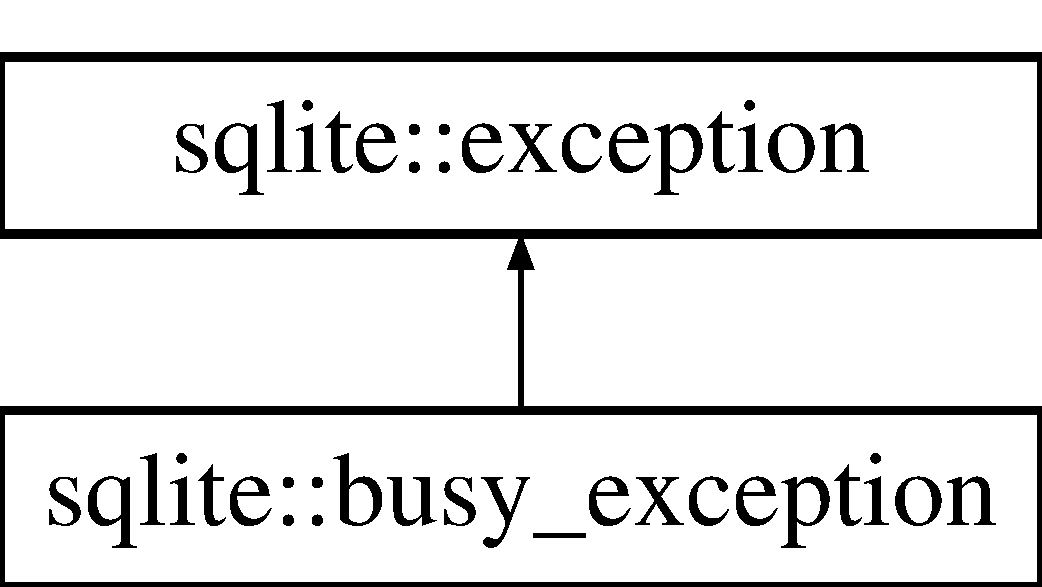
\includegraphics[height=2.000000cm]{a00003}
\end{center}
\end{figure}


\subsection{Detailed Description}
Encapsulation of the error code and message from S\-Q\-Lite3, based on std\-::runtime\-\_\-error. 



Definition at line 12 of file Exception.\-h.



The documentation for this class was generated from the following file\-:\begin{DoxyCompactItemize}
\item 
src/Exception.\-h\end{DoxyCompactItemize}

\hypertarget{a00004}{\section{sqlite\-:\-:dbconnection Class Reference}
\label{a00004}\index{sqlite\-::dbconnection@{sqlite\-::dbconnection}}
}


Class that represents a connection to a database.  




{\ttfamily \#include $<$D\-B\-Connection.\-h$>$}

\subsection*{Public Member Functions}
\begin{DoxyCompactItemize}
\item 
\hypertarget{a00004_a1cfe02390c4b08e78787120edaed6ab7}{\hyperlink{a00004_a1cfe02390c4b08e78787120edaed6ab7}{dbconnection} () noexcept}\label{a00004_a1cfe02390c4b08e78787120edaed6ab7}

\begin{DoxyCompactList}\small\item\em Default constructor. \end{DoxyCompactList}\item 
\hyperlink{a00004_a6c17517eb1631c15b64a0c54dd5355ca}{dbconnection} (const \hyperlink{a00004}{dbconnection} \&other) noexcept
\begin{DoxyCompactList}\small\item\em Copy constructor. \end{DoxyCompactList}\item 
\hyperlink{a00004_a31b78d1afbfc6147319eabb9f0e23bc5}{dbconnection} (\hyperlink{a00004}{dbconnection} \&\&other) noexcept
\begin{DoxyCompactList}\small\item\em Copy constructor. \end{DoxyCompactList}\item 
\hyperlink{a00004_a65e20f08669b49b018614cddd47efa77}{dbconnection} (const std\-::string \&filename, openmode mode=openmode\-::read\-\_\-write$\vert$openmode\-::create, const std\-::chrono\-::milliseconds timeout=D\-E\-F\-A\-U\-L\-T\-\_\-\-T\-I\-M\-E\-O\-U\-T)
\begin{DoxyCompactList}\small\item\em Open the provided database U\-T\-F-\/8 filename. \end{DoxyCompactList}\item 
\hyperlink{a00004_a4de544133c1a430855624c94986ed16c}{dbconnection} (const std\-::string \&filename, const std\-::chrono\-::milliseconds timeout)
\begin{DoxyCompactList}\small\item\em Open the provided database U\-T\-F-\/8 filename. \end{DoxyCompactList}\item 
\hyperlink{a00004_a1ac3a4126d0c5da0773f14e9ac443678}{dbconnection} (const std\-::u16string \&filename, const std\-::chrono\-::milliseconds timeout=D\-E\-F\-A\-U\-L\-T\-\_\-\-T\-I\-M\-E\-O\-U\-T)
\begin{DoxyCompactList}\small\item\em Open the provided database U\-T\-F-\/16 filename. \end{DoxyCompactList}\item 
\hyperlink{a00004}{dbconnection} \& \hyperlink{a00004_ae7c52ec41d3dfb7f4c8a521af7673bde}{operator=} (const \hyperlink{a00004}{dbconnection} \&other) noexcept
\begin{DoxyCompactList}\small\item\em Copy assignment operator. \end{DoxyCompactList}\item 
\hyperlink{a00004}{dbconnection} \& \hyperlink{a00004_abd91c727842023d54fdb64e6e2e9ac3c}{operator=} (\hyperlink{a00004}{dbconnection} \&\&other) noexcept
\begin{DoxyCompactList}\small\item\em Move assignment operator. \end{DoxyCompactList}\item 
\hyperlink{a00009}{sqlite\-::mutex} \hyperlink{a00004_afa13431e657c74ba7beee63fa70eeb93}{mutex} ()
\begin{DoxyCompactList}\small\item\em Returns a mutex that serializes access to the database. \end{DoxyCompactList}\item 
\hyperlink{a00004_a8c0e145b3687659ec0f76949174651e0}{operator bool} () const noexcept
\begin{DoxyCompactList}\small\item\em Specifies if the dbconnection has a open database connection. \end{DoxyCompactList}\item 
\hypertarget{a00004_a1a9b022293133991f265c10c1f50800b}{sqlite3 $\ast$ \hyperlink{a00004_a1a9b022293133991f265c10c1f50800b}{handle} () const noexcept}\label{a00004_a1a9b022293133991f265c10c1f50800b}

\begin{DoxyCompactList}\small\item\em Returns pointer to the underlying \char`\"{}sqlite3\char`\"{} object. \end{DoxyCompactList}\item 
void \hyperlink{a00004_a84da73c4ff1b162624da3e252c2a86c8}{open} (const std\-::string \&filename, openmode mode=openmode\-::read\-\_\-write$\vert$openmode\-::create)
\begin{DoxyCompactList}\small\item\em Open an \hyperlink{a00038}{S\-Q\-Lite} database file as specified by the filename argument. \end{DoxyCompactList}\item 
void \hyperlink{a00004_ac31065d17d9cbe1e1b3021bf11ff0229}{open} (const std\-::u16string \&filename)
\begin{DoxyCompactList}\small\item\em Open an \hyperlink{a00038}{S\-Q\-Lite} database file as specified by the filname argument. \end{DoxyCompactList}\item 
long long \hyperlink{a00004_add860c9b2c630bcfc178e3a7e878ea1b}{row\-\_\-id} () const noexcept
\begin{DoxyCompactList}\small\item\em Returns the rowid of the most recent successful \char`\"{}\-I\-N\-S\-E\-R\-T\char`\"{} into a rowid table or virtual table on database connection. \end{DoxyCompactList}\item 
{\footnotesize template$<$typename F $>$ }\\void \hyperlink{a00004_a3cc15c8f2784e6b706a5992c8014c2dd}{create\-\_\-general\-\_\-function} (const std\-::string \&name, F \&\&function, int is\-\_\-deterministic=false, const textencoding encoding=textencoding\-::utf8, int nargs=-\/1)
\begin{DoxyCompactList}\small\item\em Used to add S\-Q\-L functions or redefine the behavior of existing S\-Q\-L functions. \end{DoxyCompactList}\item 
{\footnotesize template$<$typename F $>$ }\\void \hyperlink{a00004_ad42c081096ec64f35710aa021f2f4b56}{create\-\_\-function} (const std\-::string \&name, F \&\&function, bool is\-\_\-deterministic=false, const textencoding encoding=textencoding\-::utf8)
\begin{DoxyCompactList}\small\item\em Used to add S\-Q\-L functions or redefine the behavior of existing S\-Q\-L functions. \end{DoxyCompactList}\item 
{\footnotesize template$<$typename A $>$ }\\void \hyperlink{a00004_ab3e54d1eef4c27734e45a61d27be386b}{create\-\_\-aggregate} (const std\-::string \&name, bool is\-\_\-deterministic=false, const textencoding encoding=textencoding\-::utf8)
\begin{DoxyCompactList}\small\item\em Used to add S\-Q\-L aggregate functions or redefine the behavior of existing S\-Q\-L aggregate functions. \end{DoxyCompactList}\item 
{\footnotesize template$<$typename F $>$ }\\void \hyperlink{a00004_ab8c7b939c1b6d41259aefa3b7475f3bd}{create\-\_\-collation} (const std\-::string \&name, F \&\&function, const textencoding encoding=textencoding\-::utf8)
\begin{DoxyCompactList}\small\item\em Used to add an S\-Q\-L collation or redefine the behavior of existing S\-Q\-L collations. \end{DoxyCompactList}\end{DoxyCompactItemize}
\subsection*{Static Public Member Functions}
\begin{DoxyCompactItemize}
\item 
static \hyperlink{a00004}{dbconnection} \hyperlink{a00004_adc0120a0d5d39eabcffb7d641b0c40dd}{memory} ()
\begin{DoxyCompactList}\small\item\em Create a purely in memory database. \end{DoxyCompactList}\item 
static \hyperlink{a00004}{dbconnection} \hyperlink{a00004_abe5e2bf211f18f2f358f4293d3064679}{wide\-\_\-memory} ()
\begin{DoxyCompactList}\small\item\em Create a purely in memory database with U\-T\-F-\/16 as the native byte order. \end{DoxyCompactList}\end{DoxyCompactItemize}


\subsection{Detailed Description}
Class that represents a connection to a database. 

The class dbconnection is a wrapper around the \char`\"{}sqlite3\char`\"{} structure. 

Definition at line 24 of file D\-B\-Connection.\-h.



\subsection{Constructor \& Destructor Documentation}
\hypertarget{a00004_a6c17517eb1631c15b64a0c54dd5355ca}{\index{sqlite\-::dbconnection@{sqlite\-::dbconnection}!dbconnection@{dbconnection}}
\index{dbconnection@{dbconnection}!sqlite::dbconnection@{sqlite\-::dbconnection}}
\subsubsection[{dbconnection}]{\setlength{\rightskip}{0pt plus 5cm}sqlite\-::dbconnection\-::dbconnection (
\begin{DoxyParamCaption}
\item[{const {\bf dbconnection} \&}]{other}
\end{DoxyParamCaption}
)\hspace{0.3cm}{\ttfamily [noexcept]}}}\label{a00004_a6c17517eb1631c15b64a0c54dd5355ca}


Copy constructor. 


\begin{DoxyParams}[1]{Parameters}
\mbox{\tt in}  & {\em other} & another dbconnection object to use as source to initialize object with. \\
\hline
\end{DoxyParams}


Definition at line 11 of file D\-B\-Connection.\-cpp.

\hypertarget{a00004_a31b78d1afbfc6147319eabb9f0e23bc5}{\index{sqlite\-::dbconnection@{sqlite\-::dbconnection}!dbconnection@{dbconnection}}
\index{dbconnection@{dbconnection}!sqlite::dbconnection@{sqlite\-::dbconnection}}
\subsubsection[{dbconnection}]{\setlength{\rightskip}{0pt plus 5cm}sqlite\-::dbconnection\-::dbconnection (
\begin{DoxyParamCaption}
\item[{{\bf dbconnection} \&\&}]{other}
\end{DoxyParamCaption}
)\hspace{0.3cm}{\ttfamily [noexcept]}}}\label{a00004_a31b78d1afbfc6147319eabb9f0e23bc5}


Copy constructor. 

Constructs a dbconnection object with a copy of the contents of other using move semantics. 
\begin{DoxyParams}[1]{Parameters}
\mbox{\tt in}  & {\em other} & another dbconnection object to use as source to initialize object with. \\
\hline
\end{DoxyParams}


Definition at line 15 of file D\-B\-Connection.\-cpp.

\hypertarget{a00004_a65e20f08669b49b018614cddd47efa77}{\index{sqlite\-::dbconnection@{sqlite\-::dbconnection}!dbconnection@{dbconnection}}
\index{dbconnection@{dbconnection}!sqlite::dbconnection@{sqlite\-::dbconnection}}
\subsubsection[{dbconnection}]{\setlength{\rightskip}{0pt plus 5cm}sqlite\-::dbconnection\-::dbconnection (
\begin{DoxyParamCaption}
\item[{const std\-::string \&}]{filename, }
\item[{openmode}]{mode = {\ttfamily openmode\-:\-:read\-\_\-write~$\vert$~openmode\-:\-:create}, }
\item[{const std\-::chrono\-::milliseconds}]{timeout = {\ttfamily DEFAULT\-\_\-TIMEOUT}}
\end{DoxyParamCaption}
)}}\label{a00004_a65e20f08669b49b018614cddd47efa77}


Open the provided database U\-T\-F-\/8 filename. 


\begin{DoxyParams}[1]{Parameters}
\mbox{\tt in}  & {\em filename} & U\-T\-F-\/8 path/uri to the database database file \\
\hline
\mbox{\tt in}  & {\em mode} & file opening options specified by combination of openmode flags \\
\hline
\mbox{\tt in}  & {\em timeout} & amount of milliseconds to wait before returning \hyperlink{a00003}{sqlite\-::busy\-\_\-exception} when a table is locked \\
\hline
\end{DoxyParams}


Definition at line 35 of file D\-B\-Connection.\-cpp.

\hypertarget{a00004_a4de544133c1a430855624c94986ed16c}{\index{sqlite\-::dbconnection@{sqlite\-::dbconnection}!dbconnection@{dbconnection}}
\index{dbconnection@{dbconnection}!sqlite::dbconnection@{sqlite\-::dbconnection}}
\subsubsection[{dbconnection}]{\setlength{\rightskip}{0pt plus 5cm}sqlite\-::dbconnection\-::dbconnection (
\begin{DoxyParamCaption}
\item[{const std\-::string \&}]{filename, }
\item[{const std\-::chrono\-::milliseconds}]{timeout}
\end{DoxyParamCaption}
)}}\label{a00004_a4de544133c1a430855624c94986ed16c}


Open the provided database U\-T\-F-\/8 filename. 


\begin{DoxyParams}[1]{Parameters}
\mbox{\tt in}  & {\em filename} & U\-T\-F-\/8 path/uri to the database database file \\
\hline
\mbox{\tt in}  & {\em timeout} & amount of milliseconds to wait before returning \hyperlink{a00003}{sqlite\-::busy\-\_\-exception} when a table is locked \\
\hline
\end{DoxyParams}


Definition at line 44 of file D\-B\-Connection.\-cpp.

\hypertarget{a00004_a1ac3a4126d0c5da0773f14e9ac443678}{\index{sqlite\-::dbconnection@{sqlite\-::dbconnection}!dbconnection@{dbconnection}}
\index{dbconnection@{dbconnection}!sqlite::dbconnection@{sqlite\-::dbconnection}}
\subsubsection[{dbconnection}]{\setlength{\rightskip}{0pt plus 5cm}sqlite\-::dbconnection\-::dbconnection (
\begin{DoxyParamCaption}
\item[{const std\-::u16string \&}]{filename, }
\item[{const std\-::chrono\-::milliseconds}]{timeout = {\ttfamily DEFAULT\-\_\-TIMEOUT}}
\end{DoxyParamCaption}
)}}\label{a00004_a1ac3a4126d0c5da0773f14e9ac443678}


Open the provided database U\-T\-F-\/16 filename. 


\begin{DoxyParams}[1]{Parameters}
\mbox{\tt in}  & {\em filename} & U\-T\-F-\/16 path/uri to the database database file \\
\hline
\mbox{\tt in}  & {\em timeout} & Amount of milliseconds to wait before returning \hyperlink{a00003}{sqlite\-::busy\-\_\-exception} when a table is locked \\
\hline
\end{DoxyParams}


Definition at line 52 of file D\-B\-Connection.\-cpp.



\subsection{Member Function Documentation}
\hypertarget{a00004_ab3e54d1eef4c27734e45a61d27be386b}{\index{sqlite\-::dbconnection@{sqlite\-::dbconnection}!create\-\_\-aggregate@{create\-\_\-aggregate}}
\index{create\-\_\-aggregate@{create\-\_\-aggregate}!sqlite::dbconnection@{sqlite\-::dbconnection}}
\subsubsection[{create\-\_\-aggregate}]{\setlength{\rightskip}{0pt plus 5cm}template$<$typename A $>$ void sqlite\-::dbconnection\-::create\-\_\-aggregate (
\begin{DoxyParamCaption}
\item[{const std\-::string \&}]{name, }
\item[{bool}]{is\-\_\-deterministic = {\ttfamily false}, }
\item[{const textencoding}]{encoding = {\ttfamily textencoding\-:\-:utf8}}
\end{DoxyParamCaption}
)\hspace{0.3cm}{\ttfamily [inline]}}}\label{a00004_ab3e54d1eef4c27734e45a61d27be386b}


Used to add S\-Q\-L aggregate functions or redefine the behavior of existing S\-Q\-L aggregate functions. 


\begin{DoxyTemplParams}{Template Parameters}
{\em A} & The class to use as the aggregate function. \\
\hline
\end{DoxyTemplParams}

\begin{DoxyParams}[1]{Parameters}
\mbox{\tt in}  & {\em name} & the name of the aggregate function to be used in an S\-Q\-L query \\
\hline
\mbox{\tt in}  & {\em is\-\_\-deterministic} & specifies if the function will always return the same result given the same inputs within a single S\-Q\-L statement. \\
\hline
\mbox{\tt in}  & {\em encoding} & specifies the test encoding the S\-Q\-L function prefers for its parameters \\
\hline
\end{DoxyParams}


Definition at line 203 of file D\-B\-Connection.\-h.

\hypertarget{a00004_ab8c7b939c1b6d41259aefa3b7475f3bd}{\index{sqlite\-::dbconnection@{sqlite\-::dbconnection}!create\-\_\-collation@{create\-\_\-collation}}
\index{create\-\_\-collation@{create\-\_\-collation}!sqlite::dbconnection@{sqlite\-::dbconnection}}
\subsubsection[{create\-\_\-collation}]{\setlength{\rightskip}{0pt plus 5cm}template$<$typename F $>$ void sqlite\-::dbconnection\-::create\-\_\-collation (
\begin{DoxyParamCaption}
\item[{const std\-::string \&}]{name, }
\item[{F \&\&}]{function, }
\item[{const textencoding}]{encoding = {\ttfamily textencoding\-:\-:utf8}}
\end{DoxyParamCaption}
)\hspace{0.3cm}{\ttfamily [inline]}}}\label{a00004_ab8c7b939c1b6d41259aefa3b7475f3bd}


Used to add an S\-Q\-L collation or redefine the behavior of existing S\-Q\-L collations. 


\begin{DoxyTemplParams}{Template Parameters}
{\em F} & The function type to use to create the function. \\
\hline
\end{DoxyTemplParams}

\begin{DoxyParams}[1]{Parameters}
\mbox{\tt in}  & {\em name} & the name of the function to be used in an S\-Q\-L query \\
\hline
\mbox{\tt in}  & {\em function} & the implementation to the function \\
\hline
\mbox{\tt in}  & {\em encoding} & specifies the test encoding the S\-Q\-L function prefers for its parameters \\
\hline
\end{DoxyParams}


Definition at line 237 of file D\-B\-Connection.\-h.

\hypertarget{a00004_ad42c081096ec64f35710aa021f2f4b56}{\index{sqlite\-::dbconnection@{sqlite\-::dbconnection}!create\-\_\-function@{create\-\_\-function}}
\index{create\-\_\-function@{create\-\_\-function}!sqlite::dbconnection@{sqlite\-::dbconnection}}
\subsubsection[{create\-\_\-function}]{\setlength{\rightskip}{0pt plus 5cm}template$<$typename F $>$ void sqlite\-::dbconnection\-::create\-\_\-function (
\begin{DoxyParamCaption}
\item[{const std\-::string \&}]{name, }
\item[{F \&\&}]{function, }
\item[{bool}]{is\-\_\-deterministic = {\ttfamily false}, }
\item[{const textencoding}]{encoding = {\ttfamily textencoding\-:\-:utf8}}
\end{DoxyParamCaption}
)\hspace{0.3cm}{\ttfamily [inline]}}}\label{a00004_ad42c081096ec64f35710aa021f2f4b56}


Used to add S\-Q\-L functions or redefine the behavior of existing S\-Q\-L functions. 


\begin{DoxyTemplParams}{Template Parameters}
{\em F} & The function type to use to create the function. \\
\hline
\end{DoxyTemplParams}

\begin{DoxyParams}[1]{Parameters}
\mbox{\tt in}  & {\em name} & the name of the function to be used in an S\-Q\-L query \\
\hline
\mbox{\tt in}  & {\em function} & the implementation to the function \\
\hline
\mbox{\tt in}  & {\em is\-\_\-deterministic} & specifies if the function will always return the same result given the same inputs within a single S\-Q\-L statement. \\
\hline
\mbox{\tt in}  & {\em encoding} & specifies the test encoding the S\-Q\-L function prefers for its parameters \\
\hline
\end{DoxyParams}


Definition at line 168 of file D\-B\-Connection.\-h.

\hypertarget{a00004_a3cc15c8f2784e6b706a5992c8014c2dd}{\index{sqlite\-::dbconnection@{sqlite\-::dbconnection}!create\-\_\-general\-\_\-function@{create\-\_\-general\-\_\-function}}
\index{create\-\_\-general\-\_\-function@{create\-\_\-general\-\_\-function}!sqlite::dbconnection@{sqlite\-::dbconnection}}
\subsubsection[{create\-\_\-general\-\_\-function}]{\setlength{\rightskip}{0pt plus 5cm}template$<$typename F $>$ void sqlite\-::dbconnection\-::create\-\_\-general\-\_\-function (
\begin{DoxyParamCaption}
\item[{const std\-::string \&}]{name, }
\item[{F \&\&}]{function, }
\item[{int}]{is\-\_\-deterministic = {\ttfamily false}, }
\item[{const textencoding}]{encoding = {\ttfamily textencoding\-:\-:utf8}, }
\item[{int}]{nargs = {\ttfamily -\/1}}
\end{DoxyParamCaption}
)\hspace{0.3cm}{\ttfamily [inline]}}}\label{a00004_a3cc15c8f2784e6b706a5992c8014c2dd}


Used to add S\-Q\-L functions or redefine the behavior of existing S\-Q\-L functions. 


\begin{DoxyTemplParams}{Template Parameters}
{\em F} & The function type to use to create the function. \\
\hline
\end{DoxyTemplParams}

\begin{DoxyParams}[1]{Parameters}
\mbox{\tt in}  & {\em name} & the name of the function to be used in an S\-Q\-L query \\
\hline
\mbox{\tt in}  & {\em function} & the implementation to the function \\
\hline
\mbox{\tt in}  & {\em is\-\_\-deterministic} & specifies if the function will always return the same result given the same inputs within a single S\-Q\-L statement. \\
\hline
\mbox{\tt in}  & {\em encoding} & specifies the text encoding the S\-Q\-L function prefers for its parameters. \\
\hline
\mbox{\tt in}  & {\em nargs} & the number of arguments that the S\-Q\-L function takes. -\/1 means the S\-Q\-L function can take any number of arguments. \\
\hline
\end{DoxyParams}


Definition at line 131 of file D\-B\-Connection.\-h.

\hypertarget{a00004_adc0120a0d5d39eabcffb7d641b0c40dd}{\index{sqlite\-::dbconnection@{sqlite\-::dbconnection}!memory@{memory}}
\index{memory@{memory}!sqlite::dbconnection@{sqlite\-::dbconnection}}
\subsubsection[{memory}]{\setlength{\rightskip}{0pt plus 5cm}{\bf dbconnection} sqlite\-::dbconnection\-::memory (
\begin{DoxyParamCaption}
{}
\end{DoxyParamCaption}
)\hspace{0.3cm}{\ttfamily [static]}}}\label{a00004_adc0120a0d5d39eabcffb7d641b0c40dd}


Create a purely in memory database. 

\begin{DoxyReturn}{Returns}
a purely in memory \hyperlink{a00004}{sqlite\-::dbconnection} 
\end{DoxyReturn}


Definition at line 60 of file D\-B\-Connection.\-cpp.

\hypertarget{a00004_afa13431e657c74ba7beee63fa70eeb93}{\index{sqlite\-::dbconnection@{sqlite\-::dbconnection}!mutex@{mutex}}
\index{mutex@{mutex}!sqlite::dbconnection@{sqlite\-::dbconnection}}
\subsubsection[{mutex}]{\setlength{\rightskip}{0pt plus 5cm}{\bf mutex} sqlite\-::dbconnection\-::mutex (
\begin{DoxyParamCaption}
{}
\end{DoxyParamCaption}
)}}\label{a00004_afa13431e657c74ba7beee63fa70eeb93}


Returns a mutex that serializes access to the database. 

\begin{DoxyReturn}{Returns}
A mutex object for the database connection. 
\end{DoxyReturn}


Definition at line 70 of file D\-B\-Connection.\-cpp.

\hypertarget{a00004_a84da73c4ff1b162624da3e252c2a86c8}{\index{sqlite\-::dbconnection@{sqlite\-::dbconnection}!open@{open}}
\index{open@{open}!sqlite::dbconnection@{sqlite\-::dbconnection}}
\subsubsection[{open}]{\setlength{\rightskip}{0pt plus 5cm}void sqlite\-::dbconnection\-::open (
\begin{DoxyParamCaption}
\item[{const std\-::string \&}]{filename, }
\item[{openmode}]{mode = {\ttfamily openmode\-:\-:read\-\_\-write~$\vert$~openmode\-:\-:create}}
\end{DoxyParamCaption}
)}}\label{a00004_a84da73c4ff1b162624da3e252c2a86c8}


Open an \hyperlink{a00038}{S\-Q\-Lite} database file as specified by the filename argument. 


\begin{DoxyParams}[1]{Parameters}
\mbox{\tt in}  & {\em filename} & path to \hyperlink{a00038}{S\-Q\-Lite} file \\
\hline
\mbox{\tt in}  & {\em mode} & specifies the privileges to use when opening the database. \\
\hline
\end{DoxyParams}


Definition at line 89 of file D\-B\-Connection.\-cpp.

\hypertarget{a00004_ac31065d17d9cbe1e1b3021bf11ff0229}{\index{sqlite\-::dbconnection@{sqlite\-::dbconnection}!open@{open}}
\index{open@{open}!sqlite::dbconnection@{sqlite\-::dbconnection}}
\subsubsection[{open}]{\setlength{\rightskip}{0pt plus 5cm}void sqlite\-::dbconnection\-::open (
\begin{DoxyParamCaption}
\item[{const std\-::u16string \&}]{filename}
\end{DoxyParamCaption}
)}}\label{a00004_ac31065d17d9cbe1e1b3021bf11ff0229}


Open an \hyperlink{a00038}{S\-Q\-Lite} database file as specified by the filname argument. 

The database file will have U\-T\-F-\/16 native byte order. 
\begin{DoxyParams}[1]{Parameters}
\mbox{\tt in}  & {\em filename} & path to \hyperlink{a00038}{S\-Q\-Lite} file \\
\hline
\end{DoxyParams}


Definition at line 101 of file D\-B\-Connection.\-cpp.

\hypertarget{a00004_a8c0e145b3687659ec0f76949174651e0}{\index{sqlite\-::dbconnection@{sqlite\-::dbconnection}!operator bool@{operator bool}}
\index{operator bool@{operator bool}!sqlite::dbconnection@{sqlite\-::dbconnection}}
\subsubsection[{operator bool}]{\setlength{\rightskip}{0pt plus 5cm}sqlite\-::dbconnection\-::operator bool (
\begin{DoxyParamCaption}
{}
\end{DoxyParamCaption}
) const\hspace{0.3cm}{\ttfamily [explicit]}, {\ttfamily [noexcept]}}}\label{a00004_a8c0e145b3687659ec0f76949174651e0}


Specifies if the dbconnection has a open database connection. 

\begin{DoxyReturn}{Returns}
Returns true if the dbconnection has a open database connection associated associated with it. 
\end{DoxyReturn}


Definition at line 79 of file D\-B\-Connection.\-cpp.

\hypertarget{a00004_ae7c52ec41d3dfb7f4c8a521af7673bde}{\index{sqlite\-::dbconnection@{sqlite\-::dbconnection}!operator=@{operator=}}
\index{operator=@{operator=}!sqlite::dbconnection@{sqlite\-::dbconnection}}
\subsubsection[{operator=}]{\setlength{\rightskip}{0pt plus 5cm}{\bf dbconnection} \& sqlite\-::dbconnection\-::operator= (
\begin{DoxyParamCaption}
\item[{const {\bf dbconnection} \&}]{other}
\end{DoxyParamCaption}
)\hspace{0.3cm}{\ttfamily [noexcept]}}}\label{a00004_ae7c52ec41d3dfb7f4c8a521af7673bde}


Copy assignment operator. 

Replaces the contents with those of other. 
\begin{DoxyParams}[1]{Parameters}
\mbox{\tt in}  & {\em other} & another dbconnection object to use as source to initialize object with. \\
\hline
\end{DoxyParams}
\begin{DoxyReturn}{Returns}
$\ast$this 
\end{DoxyReturn}


Definition at line 19 of file D\-B\-Connection.\-cpp.

\hypertarget{a00004_abd91c727842023d54fdb64e6e2e9ac3c}{\index{sqlite\-::dbconnection@{sqlite\-::dbconnection}!operator=@{operator=}}
\index{operator=@{operator=}!sqlite::dbconnection@{sqlite\-::dbconnection}}
\subsubsection[{operator=}]{\setlength{\rightskip}{0pt plus 5cm}{\bf dbconnection} \& sqlite\-::dbconnection\-::operator= (
\begin{DoxyParamCaption}
\item[{{\bf dbconnection} \&\&}]{other}
\end{DoxyParamCaption}
)\hspace{0.3cm}{\ttfamily [noexcept]}}}\label{a00004_abd91c727842023d54fdb64e6e2e9ac3c}


Move assignment operator. 

Replaces the contents with those of other using move semantics. 
\begin{DoxyParams}[1]{Parameters}
\mbox{\tt in}  & {\em other} & another dbconnection object to use as source to initialize object with. \\
\hline
\end{DoxyParams}
\begin{DoxyReturn}{Returns}
$\ast$this 
\end{DoxyReturn}


Definition at line 28 of file D\-B\-Connection.\-cpp.

\hypertarget{a00004_add860c9b2c630bcfc178e3a7e878ea1b}{\index{sqlite\-::dbconnection@{sqlite\-::dbconnection}!row\-\_\-id@{row\-\_\-id}}
\index{row\-\_\-id@{row\-\_\-id}!sqlite::dbconnection@{sqlite\-::dbconnection}}
\subsubsection[{row\-\_\-id}]{\setlength{\rightskip}{0pt plus 5cm}long long sqlite\-::dbconnection\-::row\-\_\-id (
\begin{DoxyParamCaption}
{}
\end{DoxyParamCaption}
) const\hspace{0.3cm}{\ttfamily [noexcept]}}}\label{a00004_add860c9b2c630bcfc178e3a7e878ea1b}


Returns the rowid of the most recent successful \char`\"{}\-I\-N\-S\-E\-R\-T\char`\"{} into a rowid table or virtual table on database connection. 

\begin{DoxyReturn}{Returns}
rowid of the most recent successful \char`\"{}\-I\-N\-S\-E\-R\-T\char`\"{} into the database, or 0 if there was none. 
\end{DoxyReturn}


Definition at line 113 of file D\-B\-Connection.\-cpp.

\hypertarget{a00004_abe5e2bf211f18f2f358f4293d3064679}{\index{sqlite\-::dbconnection@{sqlite\-::dbconnection}!wide\-\_\-memory@{wide\-\_\-memory}}
\index{wide\-\_\-memory@{wide\-\_\-memory}!sqlite::dbconnection@{sqlite\-::dbconnection}}
\subsubsection[{wide\-\_\-memory}]{\setlength{\rightskip}{0pt plus 5cm}{\bf dbconnection} sqlite\-::dbconnection\-::wide\-\_\-memory (
\begin{DoxyParamCaption}
{}
\end{DoxyParamCaption}
)\hspace{0.3cm}{\ttfamily [static]}}}\label{a00004_abe5e2bf211f18f2f358f4293d3064679}


Create a purely in memory database with U\-T\-F-\/16 as the native byte order. 

\begin{DoxyReturn}{Returns}
a purely in memory \hyperlink{a00004}{sqlite\-::dbconnection} 
\end{DoxyReturn}


Definition at line 65 of file D\-B\-Connection.\-cpp.



The documentation for this class was generated from the following files\-:\begin{DoxyCompactItemize}
\item 
src/\hyperlink{a00022}{D\-B\-Connection.\-h}\item 
src/D\-B\-Connection.\-cpp\end{DoxyCompactItemize}

\hypertarget{a00005}{\section{S\-Q\-Lite\-:\-:Mutex Class Reference}
\label{a00005}\index{S\-Q\-Lite\-::\-Mutex@{S\-Q\-Lite\-::\-Mutex}}
}


Helps with serializing access to a database connection.  




{\ttfamily \#include $<$Mutex.\-h$>$}

\subsection*{Public Member Functions}
\begin{DoxyCompactItemize}
\item 
\hypertarget{a00005_a56ba1f0c1411940ab52279497d15812a}{void \hyperlink{a00005_a56ba1f0c1411940ab52279497d15812a}{lock} () noexcept}\label{a00005_a56ba1f0c1411940ab52279497d15812a}

\begin{DoxyCompactList}\small\item\em Locks the mutex, blocks if the mutex is not available. \end{DoxyCompactList}\item 
bool \hyperlink{a00005_a95b5ebd5fef0bd37b30e3867d60389f8}{try\-Lock} () noexcept
\begin{DoxyCompactList}\small\item\em Tries to lock the mutex, returns if the mutex is not available. \end{DoxyCompactList}\item 
\hypertarget{a00005_ad9238aeb94205ac18d67c9652dcc6ef9}{void \hyperlink{a00005_ad9238aeb94205ac18d67c9652dcc6ef9}{unlock} () noexcept}\label{a00005_ad9238aeb94205ac18d67c9652dcc6ef9}

\begin{DoxyCompactList}\small\item\em Unlocks the mutex. \end{DoxyCompactList}\end{DoxyCompactItemize}


\subsection{Detailed Description}
Helps with serializing access to a database connection. 

Mutexes are only useful when threading mode is set to \char`\"{}\-Serialized\char`\"{}. 

Definition at line 12 of file Mutex.\-h.



\subsection{Member Function Documentation}
\hypertarget{a00005_a95b5ebd5fef0bd37b30e3867d60389f8}{\index{S\-Q\-Lite\-::\-Mutex@{S\-Q\-Lite\-::\-Mutex}!try\-Lock@{try\-Lock}}
\index{try\-Lock@{try\-Lock}!SQLite::Mutex@{S\-Q\-Lite\-::\-Mutex}}
\subsubsection[{try\-Lock}]{\setlength{\rightskip}{0pt plus 5cm}bool S\-Q\-Lite\-::\-Mutex\-::try\-Lock (
\begin{DoxyParamCaption}
{}
\end{DoxyParamCaption}
)\hspace{0.3cm}{\ttfamily [noexcept]}}}\label{a00005_a95b5ebd5fef0bd37b30e3867d60389f8}


Tries to lock the mutex, returns if the mutex is not available. 

\begin{DoxyReturn}{Returns}
True if able to obtain lock. False otherwise. 
\end{DoxyReturn}


Definition at line 22 of file Mutex.\-cpp.



The documentation for this class was generated from the following files\-:\begin{DoxyCompactItemize}
\item 
src/Mutex.\-h\item 
src/Mutex.\-cpp\end{DoxyCompactItemize}

\hypertarget{a00006}{\section{sqlite\-:\-:exception Class Reference}
\label{a00006}\index{sqlite\-::exception@{sqlite\-::exception}}
}


Encapsulation of the error code and message from S\-Q\-Lite3, based on std\-::runtime\-\_\-error.  




{\ttfamily \#include $<$Exception.\-h$>$}

Inheritance diagram for sqlite\-:\-:exception\-:\begin{figure}[H]
\begin{center}
\leavevmode
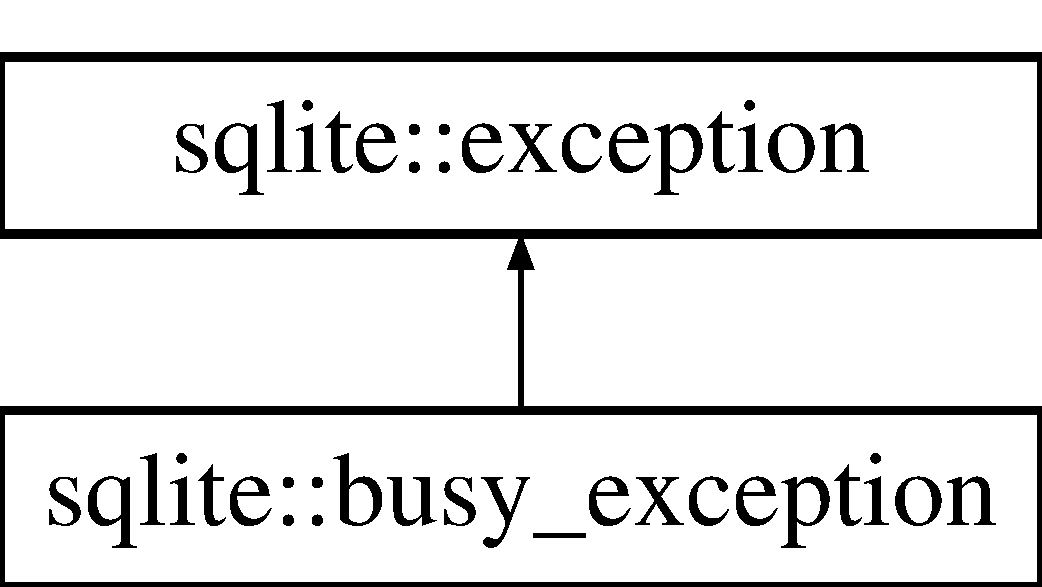
\includegraphics[height=2.000000cm]{a00006}
\end{center}
\end{figure}


\subsection{Detailed Description}
Encapsulation of the error code and message from S\-Q\-Lite3, based on std\-::runtime\-\_\-error. 



Definition at line 14 of file Exception.\-h.



The documentation for this class was generated from the following file\-:\begin{DoxyCompactItemize}
\item 
src/\hyperlink{a00024}{Exception.\-h}\end{DoxyCompactItemize}

\hypertarget{a00007}{\section{S\-Q\-Lite\-:\-:Exclusive\-Transaction Class Reference}
\label{a00007}\index{S\-Q\-Lite\-::\-Exclusive\-Transaction@{S\-Q\-Lite\-::\-Exclusive\-Transaction}}
}


R\-A\-I\-I encapsulation of the \hyperlink{a00038}{S\-Q\-Lite} exclusive transaction.  




{\ttfamily \#include $<$Transaction.\-h$>$}

Inheritance diagram for S\-Q\-Lite\-:\-:Exclusive\-Transaction\-:\begin{figure}[H]
\begin{center}
\leavevmode
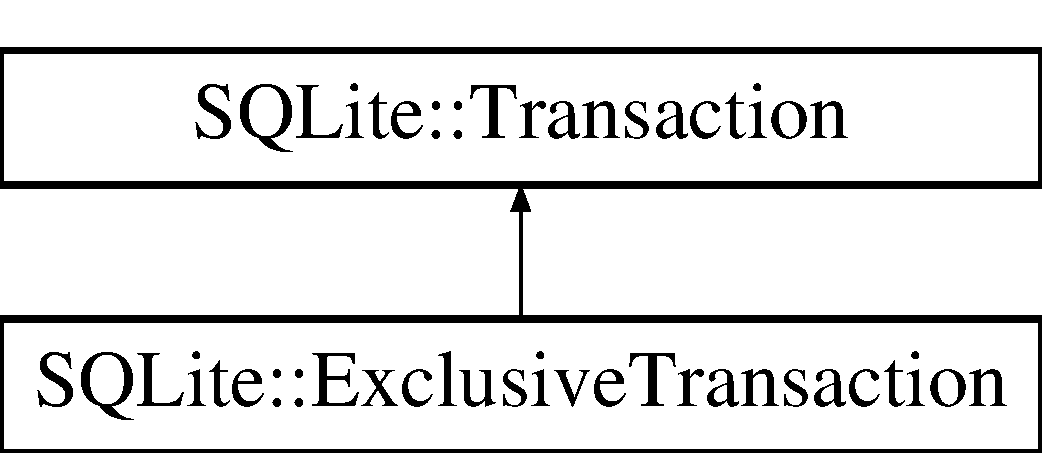
\includegraphics[height=2.000000cm]{a00007}
\end{center}
\end{figure}
\subsection*{Public Member Functions}
\begin{DoxyCompactItemize}
\item 
\hyperlink{a00007_a70f16f1e9764fd35b0c7e9fbf7314a1f}{Exclusive\-Transaction} (\hyperlink{a00004}{D\-B\-Connection} \&connection)
\begin{DoxyCompactList}\small\item\em Implements a strictly scope-\/based \hyperlink{a00038}{S\-Q\-Lite} exclusive transaction. \end{DoxyCompactList}\item 
\hypertarget{a00014_a9b251d84198cdc2c0208ad566fec0287}{virtual void \hyperlink{a00014_a9b251d84198cdc2c0208ad566fec0287}{commit} ()}\label{a00014_a9b251d84198cdc2c0208ad566fec0287}

\begin{DoxyCompactList}\small\item\em Commit the transaction. \end{DoxyCompactList}\end{DoxyCompactItemize}


\subsection{Detailed Description}
R\-A\-I\-I encapsulation of the \hyperlink{a00038}{S\-Q\-Lite} exclusive transaction. 

Definition at line 83 of file Transaction.\-h.



\subsection{Constructor \& Destructor Documentation}
\hypertarget{a00007_a70f16f1e9764fd35b0c7e9fbf7314a1f}{\index{S\-Q\-Lite\-::\-Exclusive\-Transaction@{S\-Q\-Lite\-::\-Exclusive\-Transaction}!Exclusive\-Transaction@{Exclusive\-Transaction}}
\index{Exclusive\-Transaction@{Exclusive\-Transaction}!SQLite::ExclusiveTransaction@{S\-Q\-Lite\-::\-Exclusive\-Transaction}}
\subsubsection[{Exclusive\-Transaction}]{\setlength{\rightskip}{0pt plus 5cm}S\-Q\-Lite\-::\-Exclusive\-Transaction\-::\-Exclusive\-Transaction (
\begin{DoxyParamCaption}
\item[{{\bf D\-B\-Connection} \&}]{connection}
\end{DoxyParamCaption}
)\hspace{0.3cm}{\ttfamily [inline]}}}\label{a00007_a70f16f1e9764fd35b0c7e9fbf7314a1f}


Implements a strictly scope-\/based \hyperlink{a00038}{S\-Q\-Lite} exclusive transaction. 


\begin{DoxyParams}[1]{Parameters}
\mbox{\tt in}  & {\em connection} & the database connection to begin the transaction on \\
\hline
\end{DoxyParams}


Definition at line 89 of file Transaction.\-h.



The documentation for this class was generated from the following file\-:\begin{DoxyCompactItemize}
\item 
src/\hyperlink{a00034}{Transaction.\-h}\end{DoxyCompactItemize}

\hypertarget{a00008}{\section{sqlite\-:\-:immediate\-\_\-transaction Class Reference}
\label{a00008}\index{sqlite\-::immediate\-\_\-transaction@{sqlite\-::immediate\-\_\-transaction}}
}


R\-A\-I\-I encapsulation of the S\-Q\-Lite immediate transaction.  




{\ttfamily \#include $<$Transaction.\-h$>$}

Inheritance diagram for sqlite\-:\-:immediate\-\_\-transaction\-:\begin{figure}[H]
\begin{center}
\leavevmode
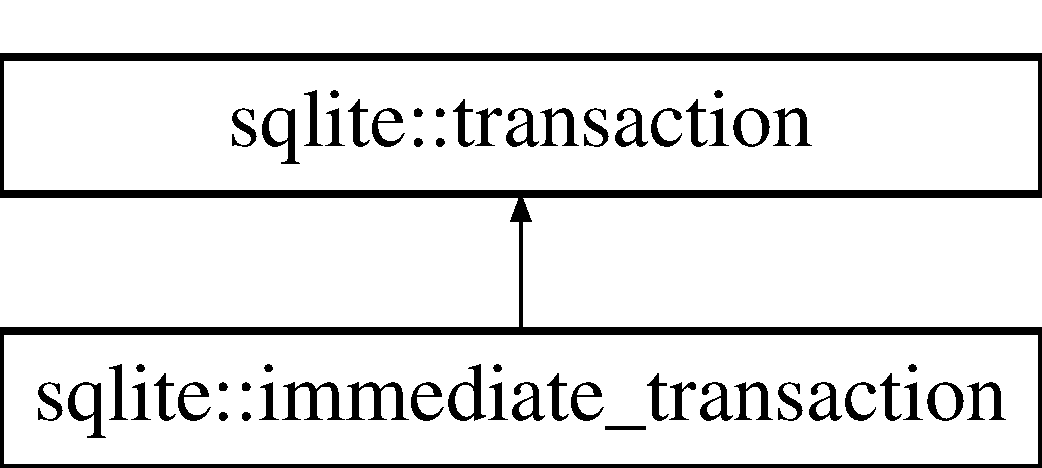
\includegraphics[height=2.000000cm]{a00008}
\end{center}
\end{figure}
\subsection*{Public Member Functions}
\begin{DoxyCompactItemize}
\item 
\hyperlink{a00008_a17924d6e15666b8340ee8aab9a88e0d1}{immediate\-\_\-transaction} (\hyperlink{a00004}{dbconnection} \&connection)
\begin{DoxyCompactList}\small\item\em Implements a strictly scope-\/based S\-Q\-Lite immediate transaction. \end{DoxyCompactList}\item 
\hypertarget{a00014_abe219dd0bf949d569381f9830c7b2d1a}{virtual void \hyperlink{a00014_abe219dd0bf949d569381f9830c7b2d1a}{commit} ()}\label{a00014_abe219dd0bf949d569381f9830c7b2d1a}

\begin{DoxyCompactList}\small\item\em Commit the transaction. \end{DoxyCompactList}\end{DoxyCompactItemize}


\subsection{Detailed Description}
R\-A\-I\-I encapsulation of the S\-Q\-Lite immediate transaction. 

Definition at line 70 of file Transaction.\-h.



\subsection{Constructor \& Destructor Documentation}
\hypertarget{a00008_a17924d6e15666b8340ee8aab9a88e0d1}{\index{sqlite\-::immediate\-\_\-transaction@{sqlite\-::immediate\-\_\-transaction}!immediate\-\_\-transaction@{immediate\-\_\-transaction}}
\index{immediate\-\_\-transaction@{immediate\-\_\-transaction}!sqlite::immediate_transaction@{sqlite\-::immediate\-\_\-transaction}}
\subsubsection[{immediate\-\_\-transaction}]{\setlength{\rightskip}{0pt plus 5cm}sqlite\-::immediate\-\_\-transaction\-::immediate\-\_\-transaction (
\begin{DoxyParamCaption}
\item[{{\bf dbconnection} \&}]{connection}
\end{DoxyParamCaption}
)\hspace{0.3cm}{\ttfamily [inline]}}}\label{a00008_a17924d6e15666b8340ee8aab9a88e0d1}


Implements a strictly scope-\/based S\-Q\-Lite immediate transaction. 


\begin{DoxyParams}[1]{Parameters}
\mbox{\tt in}  & {\em connection} & the database connection to begin the transaction on \\
\hline
\end{DoxyParams}


Definition at line 76 of file Transaction.\-h.



The documentation for this class was generated from the following file\-:\begin{DoxyCompactItemize}
\item 
src/\hyperlink{a00034}{Transaction.\-h}\end{DoxyCompactItemize}

\hypertarget{a00009}{\section{S\-Q\-Lite\-:\-:Transaction Class Reference}
\label{a00009}\index{S\-Q\-Lite\-::\-Transaction@{S\-Q\-Lite\-::\-Transaction}}
}


R\-A\-I\-I encapsulation of the S\-Q\-Lite Transactions.  




{\ttfamily \#include $<$Transaction.\-h$>$}



Inherited by S\-Q\-Lite\-::\-Deferred\-Transaction, S\-Q\-Lite\-::\-Exclusive\-Transaction, and S\-Q\-Lite\-::\-Immediate\-Transaction.

\subsection*{Public Member Functions}
\begin{DoxyCompactItemize}
\item 
\hyperlink{a00009_a27add1a1db2dd8cd5935c78a63ad556b}{Transaction} (\hyperlink{a00002}{D\-B\-Connection} \&connection, const Transaction\-Type type)
\begin{DoxyCompactList}\small\item\em Begins the S\-Q\-Lite transaction. \end{DoxyCompactList}\item 
\hypertarget{a00009_a43c5e67a10b9698b7f6dad73539feb94}{virtual \hyperlink{a00009_a43c5e67a10b9698b7f6dad73539feb94}{$\sim$\-Transaction} () noexcept}\label{a00009_a43c5e67a10b9698b7f6dad73539feb94}

\begin{DoxyCompactList}\small\item\em Safely rollback the transaction if it has not been commited. \end{DoxyCompactList}\item 
\hypertarget{a00009_a9b251d84198cdc2c0208ad566fec0287}{virtual void \hyperlink{a00009_a9b251d84198cdc2c0208ad566fec0287}{commit} ()}\label{a00009_a9b251d84198cdc2c0208ad566fec0287}

\begin{DoxyCompactList}\small\item\em Commit the transaction. \end{DoxyCompactList}\end{DoxyCompactItemize}


\subsection{Detailed Description}
R\-A\-I\-I encapsulation of the S\-Q\-Lite Transactions. 

Definition at line 21 of file Transaction.\-h.



\subsection{Constructor \& Destructor Documentation}
\hypertarget{a00009_a27add1a1db2dd8cd5935c78a63ad556b}{\index{S\-Q\-Lite\-::\-Transaction@{S\-Q\-Lite\-::\-Transaction}!Transaction@{Transaction}}
\index{Transaction@{Transaction}!SQLite::Transaction@{S\-Q\-Lite\-::\-Transaction}}
\subsubsection[{Transaction}]{\setlength{\rightskip}{0pt plus 5cm}S\-Q\-Lite\-::\-Transaction\-::\-Transaction (
\begin{DoxyParamCaption}
\item[{{\bf D\-B\-Connection} \&}]{connection, }
\item[{const Transaction\-Type}]{type}
\end{DoxyParamCaption}
)}}\label{a00009_a27add1a1db2dd8cd5935c78a63ad556b}


Begins the S\-Q\-Lite transaction. 


\begin{DoxyParams}[1]{Parameters}
\mbox{\tt in}  & {\em connection} & the database connection to begin the transaction on \\
\hline
\end{DoxyParams}


Definition at line 10 of file Transaction.\-cpp.



The documentation for this class was generated from the following files\-:\begin{DoxyCompactItemize}
\item 
src/Transaction.\-h\item 
src/Transaction.\-cpp\end{DoxyCompactItemize}

\hypertarget{a00010}{\section{S\-Q\-Lite\-:\-:Reader$<$ T $>$ Class Template Reference}
\label{a00010}\index{S\-Q\-Lite\-::\-Reader$<$ T $>$@{S\-Q\-Lite\-::\-Reader$<$ T $>$}}
}


Base class used to help with reading \char`\"{}sqlite3\-\_\-stmt\char`\"{} information.  




{\ttfamily \#include $<$Statement.\-h$>$}

\subsection*{Public Member Functions}
\begin{DoxyCompactItemize}
\item 
int \hyperlink{a00010_a82c5bc45048b8328a2fcc9bb4ff975f2}{get\-Int} (const int column) const noexcept
\begin{DoxyCompactList}\small\item\em Returns the specified column value as an integer. \end{DoxyCompactList}\item 
int \hyperlink{a00010_a87dd8234c2bd5f19466813f8a68ab80a}{get\-Int} (const std\-::string \&name) const noexcept
\begin{DoxyCompactList}\small\item\em Returns the specified column value as an integer. \end{DoxyCompactList}\item 
int64\-\_\-t \hyperlink{a00010_adb7b9705a4638d6d5af5ca26dfa474ff}{get\-Int64} (const int column) const noexcept
\begin{DoxyCompactList}\small\item\em Returns the specified column value as a 64-\/bit integer. \end{DoxyCompactList}\item 
int64\-\_\-t \hyperlink{a00010_aea6d24bb9247bfc52fe77d62be961dd2}{get\-Int64} (const std\-::string \&name) const noexcept
\begin{DoxyCompactList}\small\item\em Returns the specified column value as a 64-\/bit integer. \end{DoxyCompactList}\item 
unsigned int \hyperlink{a00010_a971fb706b9215a89532ac48640f94832}{get\-U\-Int} (const int column) const noexcept
\begin{DoxyCompactList}\small\item\em Returns the specified column value as an unsigned integer. \end{DoxyCompactList}\item 
unsigned int \hyperlink{a00010_a18315a8379249158c3f827441e8f6de0}{get\-U\-Int} (const std\-::string \&name) const noexcept
\begin{DoxyCompactList}\small\item\em Returns the specified column value as an unsigned integer. \end{DoxyCompactList}\item 
double \hyperlink{a00010_a679e56078c78e01c99fa08ad0b7ee782}{get\-Double} (const int column) const noexcept
\begin{DoxyCompactList}\small\item\em Returns the specified column value as a double. \end{DoxyCompactList}\item 
double \hyperlink{a00010_a45e9dd813439e8cda7608e18c1ccce5f}{get\-Double} (const std\-::string \&name) const noexcept
\begin{DoxyCompactList}\small\item\em Returns the specified column value as a double. \end{DoxyCompactList}\item 
const \hyperlink{a00002}{Blob} \hyperlink{a00010_a80028dc9f221648fe2398b40bd380c31}{get\-Blob} (const int column) const noexcept
\begin{DoxyCompactList}\small\item\em Returns the specified column value as a \hyperlink{a00002}{Blob} object. \end{DoxyCompactList}\item 
const \hyperlink{a00002}{Blob} \hyperlink{a00010_a4e50d9ec365c547b5edb7d062aeba72b}{get\-Blob} (const std\-::string \&name) const noexcept
\begin{DoxyCompactList}\small\item\em Returns the specified column value as a \hyperlink{a00002}{Blob} object. \end{DoxyCompactList}\item 
const std\-::string \hyperlink{a00010_a0920d021f6962f75e7b555e3f20fc0fc}{get\-String} (const int column) const noexcept
\begin{DoxyCompactList}\small\item\em Returns the specified column value as a string. \end{DoxyCompactList}\item 
const std\-::string \hyperlink{a00010_a44f9f5da46aa91b869fe26a188e803fa}{get\-String} (const std\-::string \&name) const noexcept
\begin{DoxyCompactList}\small\item\em Returns the specified column value as a string. \end{DoxyCompactList}\item 
const std\-::u16string \hyperlink{a00010_a2b48f9e2ffbcfe787d85b4372a7ee29d}{get\-U16\-String} (const int column) const noexcept
\begin{DoxyCompactList}\small\item\em Returns the specified column value as a U\-T\-F-\/16 string. \end{DoxyCompactList}\item 
const std\-::u16string \hyperlink{a00010_ad6024ad6e74ee1ac47ad0ce79f905026}{get\-U16\-String} (const std\-::string \&name) const noexcept
\begin{DoxyCompactList}\small\item\em Returns the specified column value as a U\-T\-F-\/16 string. \end{DoxyCompactList}\item 
\hyperlink{a00015}{Value} \hyperlink{a00010_a41fcbc5da6eb3fe6fc75e4faed208fc6}{get\-Value} (const int column) const noexcept
\begin{DoxyCompactList}\small\item\em Returns the specified column value as a \hyperlink{a00015}{Value} object. \end{DoxyCompactList}\item 
\hyperlink{a00015}{Value} \hyperlink{a00010_ad352a7124ee46d756462c8a1b014599a}{get\-Value} (const std\-::string \&name) const 
\begin{DoxyCompactList}\small\item\em Returns the specified column value as a \hyperlink{a00015}{Value} object. \end{DoxyCompactList}\item 
int \hyperlink{a00010_aeb571e9157ef46c42ed48fc229b7842d}{get\-Bytes} (const int column) const noexcept
\begin{DoxyCompactList}\small\item\em Returns the size in bytes of the column value. \end{DoxyCompactList}\item 
int \hyperlink{a00010_ad183a562774f9590273bf35c6e232a1a}{get\-Bytes} (const std\-::string \&name) const noexcept
\begin{DoxyCompactList}\small\item\em Returns the size in bytes of the column value. \end{DoxyCompactList}\item 
\hyperlink{a00038_ad7a8ff5f375eca25eb6e3a51d746a04c}{Type} \hyperlink{a00010_a0450ea397b1a9d8dd636b82c8757d33e}{get\-Type} (const int column) const noexcept
\begin{DoxyCompactList}\small\item\em Returns the type of the specified column. \end{DoxyCompactList}\item 
\hyperlink{a00038_ad7a8ff5f375eca25eb6e3a51d746a04c}{Type} \hyperlink{a00010_ae4f049a45c69b9e1bf6db4cf63699f64}{get\-Type} (const std\-::string \&name) const noexcept
\begin{DoxyCompactList}\small\item\em Returns the type of the specified column. \end{DoxyCompactList}\item 
int \hyperlink{a00010_a9e6b9d0d99dea8964a34a3c2f08e99bc}{get\-Column\-Count} () const noexcept
\begin{DoxyCompactList}\small\item\em Returns the number of columns in the result set returned by the prepared statement. \end{DoxyCompactList}\item 
const char $\ast$ \hyperlink{a00010_a5004961d65336631d45de411ffb87cd5}{get\-Column\-Name} (const int index) const noexcept
\begin{DoxyCompactList}\small\item\em Returns the name assigned to a particular column. \end{DoxyCompactList}\item 
const char16\-\_\-t $\ast$ \hyperlink{a00010_af46d30137ad020b1e22ad703810ea002}{get\-Column\-Wide\-Name} (const int index) const noexcept
\begin{DoxyCompactList}\small\item\em Returns the name assigned to a particular column. \end{DoxyCompactList}\item 
int \hyperlink{a00010_ae7eaa050a97cda893e9737bca416f0cb}{get\-Column\-Index} (const std\-::string \&name) const 
\begin{DoxyCompactList}\small\item\em Returns the position of a column with the specified name. \end{DoxyCompactList}\end{DoxyCompactItemize}


\subsection{Detailed Description}
\subsubsection*{template$<$typename T$>$class S\-Q\-Lite\-::\-Reader$<$ T $>$}

Base class used to help with reading \char`\"{}sqlite3\-\_\-stmt\char`\"{} information. 

This class is meant to be inherited from. 

Definition at line 30 of file Statement.\-h.



\subsection{Member Function Documentation}
\hypertarget{a00010_a80028dc9f221648fe2398b40bd380c31}{\index{S\-Q\-Lite\-::\-Reader@{S\-Q\-Lite\-::\-Reader}!get\-Blob@{get\-Blob}}
\index{get\-Blob@{get\-Blob}!SQLite::Reader@{S\-Q\-Lite\-::\-Reader}}
\subsubsection[{get\-Blob}]{\setlength{\rightskip}{0pt plus 5cm}template$<$typename T$>$ const {\bf Blob} {\bf S\-Q\-Lite\-::\-Reader}$<$ T $>$\-::get\-Blob (
\begin{DoxyParamCaption}
\item[{const int}]{column}
\end{DoxyParamCaption}
) const\hspace{0.3cm}{\ttfamily [inline]}, {\ttfamily [noexcept]}}}\label{a00010_a80028dc9f221648fe2398b40bd380c31}


Returns the specified column value as a \hyperlink{a00002}{Blob} object. 


\begin{DoxyParams}[1]{Parameters}
\mbox{\tt in}  & {\em column} & position of the column to return \\
\hline
\end{DoxyParams}
\begin{DoxyReturn}{Returns}
value of column as integer 
\end{DoxyReturn}


Definition at line 116 of file Statement.\-h.

\hypertarget{a00010_a4e50d9ec365c547b5edb7d062aeba72b}{\index{S\-Q\-Lite\-::\-Reader@{S\-Q\-Lite\-::\-Reader}!get\-Blob@{get\-Blob}}
\index{get\-Blob@{get\-Blob}!SQLite::Reader@{S\-Q\-Lite\-::\-Reader}}
\subsubsection[{get\-Blob}]{\setlength{\rightskip}{0pt plus 5cm}template$<$typename T$>$ const {\bf Blob} {\bf S\-Q\-Lite\-::\-Reader}$<$ T $>$\-::get\-Blob (
\begin{DoxyParamCaption}
\item[{const std\-::string \&}]{name}
\end{DoxyParamCaption}
) const\hspace{0.3cm}{\ttfamily [inline]}, {\ttfamily [noexcept]}}}\label{a00010_a4e50d9ec365c547b5edb7d062aeba72b}


Returns the specified column value as a \hyperlink{a00002}{Blob} object. 


\begin{DoxyParams}[1]{Parameters}
\mbox{\tt in}  & {\em name} & name of the column to return \\
\hline
\end{DoxyParams}
\begin{DoxyReturn}{Returns}
value of column as integer 
\end{DoxyReturn}


Definition at line 126 of file Statement.\-h.

\hypertarget{a00010_aeb571e9157ef46c42ed48fc229b7842d}{\index{S\-Q\-Lite\-::\-Reader@{S\-Q\-Lite\-::\-Reader}!get\-Bytes@{get\-Bytes}}
\index{get\-Bytes@{get\-Bytes}!SQLite::Reader@{S\-Q\-Lite\-::\-Reader}}
\subsubsection[{get\-Bytes}]{\setlength{\rightskip}{0pt plus 5cm}template$<$typename T$>$ int {\bf S\-Q\-Lite\-::\-Reader}$<$ T $>$\-::get\-Bytes (
\begin{DoxyParamCaption}
\item[{const int}]{column}
\end{DoxyParamCaption}
) const\hspace{0.3cm}{\ttfamily [inline]}, {\ttfamily [noexcept]}}}\label{a00010_aeb571e9157ef46c42ed48fc229b7842d}


Returns the size in bytes of the column value. 


\begin{DoxyParams}[1]{Parameters}
\mbox{\tt in}  & {\em column} & position of the column to return \\
\hline
\end{DoxyParams}
\begin{DoxyReturn}{Returns}
the size in bytes of the column value 
\end{DoxyReturn}


Definition at line 196 of file Statement.\-h.

\hypertarget{a00010_ad183a562774f9590273bf35c6e232a1a}{\index{S\-Q\-Lite\-::\-Reader@{S\-Q\-Lite\-::\-Reader}!get\-Bytes@{get\-Bytes}}
\index{get\-Bytes@{get\-Bytes}!SQLite::Reader@{S\-Q\-Lite\-::\-Reader}}
\subsubsection[{get\-Bytes}]{\setlength{\rightskip}{0pt plus 5cm}template$<$typename T$>$ int {\bf S\-Q\-Lite\-::\-Reader}$<$ T $>$\-::get\-Bytes (
\begin{DoxyParamCaption}
\item[{const std\-::string \&}]{name}
\end{DoxyParamCaption}
) const\hspace{0.3cm}{\ttfamily [inline]}, {\ttfamily [noexcept]}}}\label{a00010_ad183a562774f9590273bf35c6e232a1a}


Returns the size in bytes of the column value. 


\begin{DoxyParams}[1]{Parameters}
\mbox{\tt in}  & {\em name} & name of the column to return \\
\hline
\end{DoxyParams}
\begin{DoxyReturn}{Returns}
the size in bytes of the column value 
\end{DoxyReturn}


Definition at line 205 of file Statement.\-h.

\hypertarget{a00010_a9e6b9d0d99dea8964a34a3c2f08e99bc}{\index{S\-Q\-Lite\-::\-Reader@{S\-Q\-Lite\-::\-Reader}!get\-Column\-Count@{get\-Column\-Count}}
\index{get\-Column\-Count@{get\-Column\-Count}!SQLite::Reader@{S\-Q\-Lite\-::\-Reader}}
\subsubsection[{get\-Column\-Count}]{\setlength{\rightskip}{0pt plus 5cm}template$<$typename T$>$ int {\bf S\-Q\-Lite\-::\-Reader}$<$ T $>$\-::get\-Column\-Count (
\begin{DoxyParamCaption}
{}
\end{DoxyParamCaption}
) const\hspace{0.3cm}{\ttfamily [inline]}, {\ttfamily [noexcept]}}}\label{a00010_a9e6b9d0d99dea8964a34a3c2f08e99bc}


Returns the number of columns in the result set returned by the prepared statement. 

If this method returns 0, that means the prepared statment returns no data (for example an U\-P\-D\-A\-T\-E). \begin{DoxyReturn}{Returns}
The number of columns in the result set. 
\end{DoxyReturn}


Definition at line 234 of file Statement.\-h.

\hypertarget{a00010_ae7eaa050a97cda893e9737bca416f0cb}{\index{S\-Q\-Lite\-::\-Reader@{S\-Q\-Lite\-::\-Reader}!get\-Column\-Index@{get\-Column\-Index}}
\index{get\-Column\-Index@{get\-Column\-Index}!SQLite::Reader@{S\-Q\-Lite\-::\-Reader}}
\subsubsection[{get\-Column\-Index}]{\setlength{\rightskip}{0pt plus 5cm}template$<$typename T$>$ int {\bf S\-Q\-Lite\-::\-Reader}$<$ T $>$\-::get\-Column\-Index (
\begin{DoxyParamCaption}
\item[{const std\-::string \&}]{name}
\end{DoxyParamCaption}
) const\hspace{0.3cm}{\ttfamily [inline]}}}\label{a00010_ae7eaa050a97cda893e9737bca416f0cb}


Returns the position of a column with the specified name. 

\begin{DoxyReturn}{Returns}
The position of the column 
\end{DoxyReturn}

\begin{DoxyExceptions}{Exceptions}
{\em S\-Q\-Lite\-X\-X\-Exception} & if no column with specified name was found \\
\hline
\end{DoxyExceptions}


Definition at line 261 of file Statement.\-h.

\hypertarget{a00010_a5004961d65336631d45de411ffb87cd5}{\index{S\-Q\-Lite\-::\-Reader@{S\-Q\-Lite\-::\-Reader}!get\-Column\-Name@{get\-Column\-Name}}
\index{get\-Column\-Name@{get\-Column\-Name}!SQLite::Reader@{S\-Q\-Lite\-::\-Reader}}
\subsubsection[{get\-Column\-Name}]{\setlength{\rightskip}{0pt plus 5cm}template$<$typename T$>$ const char$\ast$ {\bf S\-Q\-Lite\-::\-Reader}$<$ T $>$\-::get\-Column\-Name (
\begin{DoxyParamCaption}
\item[{const int}]{index}
\end{DoxyParamCaption}
) const\hspace{0.3cm}{\ttfamily [inline]}, {\ttfamily [noexcept]}}}\label{a00010_a5004961d65336631d45de411ffb87cd5}


Returns the name assigned to a particular column. 


\begin{DoxyParams}[1]{Parameters}
\mbox{\tt in}  & {\em index} & the position of the column \\
\hline
\end{DoxyParams}
\begin{DoxyReturn}{Returns}
The name of the specified column. 
\end{DoxyReturn}


Definition at line 243 of file Statement.\-h.

\hypertarget{a00010_af46d30137ad020b1e22ad703810ea002}{\index{S\-Q\-Lite\-::\-Reader@{S\-Q\-Lite\-::\-Reader}!get\-Column\-Wide\-Name@{get\-Column\-Wide\-Name}}
\index{get\-Column\-Wide\-Name@{get\-Column\-Wide\-Name}!SQLite::Reader@{S\-Q\-Lite\-::\-Reader}}
\subsubsection[{get\-Column\-Wide\-Name}]{\setlength{\rightskip}{0pt plus 5cm}template$<$typename T$>$ const char16\-\_\-t$\ast$ {\bf S\-Q\-Lite\-::\-Reader}$<$ T $>$\-::get\-Column\-Wide\-Name (
\begin{DoxyParamCaption}
\item[{const int}]{index}
\end{DoxyParamCaption}
) const\hspace{0.3cm}{\ttfamily [inline]}, {\ttfamily [noexcept]}}}\label{a00010_af46d30137ad020b1e22ad703810ea002}


Returns the name assigned to a particular column. 


\begin{DoxyParams}[1]{Parameters}
\mbox{\tt in}  & {\em index} & the position of the column \\
\hline
\end{DoxyParams}
\begin{DoxyReturn}{Returns}
The name of the specified column. 
\end{DoxyReturn}


Definition at line 252 of file Statement.\-h.

\hypertarget{a00010_a679e56078c78e01c99fa08ad0b7ee782}{\index{S\-Q\-Lite\-::\-Reader@{S\-Q\-Lite\-::\-Reader}!get\-Double@{get\-Double}}
\index{get\-Double@{get\-Double}!SQLite::Reader@{S\-Q\-Lite\-::\-Reader}}
\subsubsection[{get\-Double}]{\setlength{\rightskip}{0pt plus 5cm}template$<$typename T$>$ double {\bf S\-Q\-Lite\-::\-Reader}$<$ T $>$\-::get\-Double (
\begin{DoxyParamCaption}
\item[{const int}]{column}
\end{DoxyParamCaption}
) const\hspace{0.3cm}{\ttfamily [inline]}, {\ttfamily [noexcept]}}}\label{a00010_a679e56078c78e01c99fa08ad0b7ee782}


Returns the specified column value as a double. 


\begin{DoxyParams}[1]{Parameters}
\mbox{\tt in}  & {\em column} & position of the column to return \\
\hline
\end{DoxyParams}
\begin{DoxyReturn}{Returns}
value of column as integer 
\end{DoxyReturn}


Definition at line 97 of file Statement.\-h.

\hypertarget{a00010_a45e9dd813439e8cda7608e18c1ccce5f}{\index{S\-Q\-Lite\-::\-Reader@{S\-Q\-Lite\-::\-Reader}!get\-Double@{get\-Double}}
\index{get\-Double@{get\-Double}!SQLite::Reader@{S\-Q\-Lite\-::\-Reader}}
\subsubsection[{get\-Double}]{\setlength{\rightskip}{0pt plus 5cm}template$<$typename T$>$ double {\bf S\-Q\-Lite\-::\-Reader}$<$ T $>$\-::get\-Double (
\begin{DoxyParamCaption}
\item[{const std\-::string \&}]{name}
\end{DoxyParamCaption}
) const\hspace{0.3cm}{\ttfamily [inline]}, {\ttfamily [noexcept]}}}\label{a00010_a45e9dd813439e8cda7608e18c1ccce5f}


Returns the specified column value as a double. 


\begin{DoxyParams}[1]{Parameters}
\mbox{\tt in}  & {\em name} & name of the column to return \\
\hline
\end{DoxyParams}
\begin{DoxyReturn}{Returns}
value of column as integer 
\end{DoxyReturn}


Definition at line 106 of file Statement.\-h.

\hypertarget{a00010_a82c5bc45048b8328a2fcc9bb4ff975f2}{\index{S\-Q\-Lite\-::\-Reader@{S\-Q\-Lite\-::\-Reader}!get\-Int@{get\-Int}}
\index{get\-Int@{get\-Int}!SQLite::Reader@{S\-Q\-Lite\-::\-Reader}}
\subsubsection[{get\-Int}]{\setlength{\rightskip}{0pt plus 5cm}template$<$typename T$>$ int {\bf S\-Q\-Lite\-::\-Reader}$<$ T $>$\-::get\-Int (
\begin{DoxyParamCaption}
\item[{const int}]{column}
\end{DoxyParamCaption}
) const\hspace{0.3cm}{\ttfamily [inline]}, {\ttfamily [noexcept]}}}\label{a00010_a82c5bc45048b8328a2fcc9bb4ff975f2}


Returns the specified column value as an integer. 


\begin{DoxyParams}[1]{Parameters}
\mbox{\tt in}  & {\em column} & position of the column to return \\
\hline
\end{DoxyParams}
\begin{DoxyReturn}{Returns}
value of column as integer 
\end{DoxyReturn}


Definition at line 40 of file Statement.\-h.

\hypertarget{a00010_a87dd8234c2bd5f19466813f8a68ab80a}{\index{S\-Q\-Lite\-::\-Reader@{S\-Q\-Lite\-::\-Reader}!get\-Int@{get\-Int}}
\index{get\-Int@{get\-Int}!SQLite::Reader@{S\-Q\-Lite\-::\-Reader}}
\subsubsection[{get\-Int}]{\setlength{\rightskip}{0pt plus 5cm}template$<$typename T$>$ int {\bf S\-Q\-Lite\-::\-Reader}$<$ T $>$\-::get\-Int (
\begin{DoxyParamCaption}
\item[{const std\-::string \&}]{name}
\end{DoxyParamCaption}
) const\hspace{0.3cm}{\ttfamily [inline]}, {\ttfamily [noexcept]}}}\label{a00010_a87dd8234c2bd5f19466813f8a68ab80a}


Returns the specified column value as an integer. 


\begin{DoxyParams}[1]{Parameters}
\mbox{\tt in}  & {\em name} & name of the column to return \\
\hline
\end{DoxyParams}
\begin{DoxyReturn}{Returns}
value of column as integer 
\end{DoxyReturn}


Definition at line 49 of file Statement.\-h.

\hypertarget{a00010_adb7b9705a4638d6d5af5ca26dfa474ff}{\index{S\-Q\-Lite\-::\-Reader@{S\-Q\-Lite\-::\-Reader}!get\-Int64@{get\-Int64}}
\index{get\-Int64@{get\-Int64}!SQLite::Reader@{S\-Q\-Lite\-::\-Reader}}
\subsubsection[{get\-Int64}]{\setlength{\rightskip}{0pt plus 5cm}template$<$typename T$>$ int64\-\_\-t {\bf S\-Q\-Lite\-::\-Reader}$<$ T $>$\-::get\-Int64 (
\begin{DoxyParamCaption}
\item[{const int}]{column}
\end{DoxyParamCaption}
) const\hspace{0.3cm}{\ttfamily [inline]}, {\ttfamily [noexcept]}}}\label{a00010_adb7b9705a4638d6d5af5ca26dfa474ff}


Returns the specified column value as a 64-\/bit integer. 


\begin{DoxyParams}[1]{Parameters}
\mbox{\tt in}  & {\em column} & position of the column to return \\
\hline
\end{DoxyParams}
\begin{DoxyReturn}{Returns}
value of column as integer 
\end{DoxyReturn}


Definition at line 59 of file Statement.\-h.

\hypertarget{a00010_aea6d24bb9247bfc52fe77d62be961dd2}{\index{S\-Q\-Lite\-::\-Reader@{S\-Q\-Lite\-::\-Reader}!get\-Int64@{get\-Int64}}
\index{get\-Int64@{get\-Int64}!SQLite::Reader@{S\-Q\-Lite\-::\-Reader}}
\subsubsection[{get\-Int64}]{\setlength{\rightskip}{0pt plus 5cm}template$<$typename T$>$ int64\-\_\-t {\bf S\-Q\-Lite\-::\-Reader}$<$ T $>$\-::get\-Int64 (
\begin{DoxyParamCaption}
\item[{const std\-::string \&}]{name}
\end{DoxyParamCaption}
) const\hspace{0.3cm}{\ttfamily [inline]}, {\ttfamily [noexcept]}}}\label{a00010_aea6d24bb9247bfc52fe77d62be961dd2}


Returns the specified column value as a 64-\/bit integer. 


\begin{DoxyParams}[1]{Parameters}
\mbox{\tt in}  & {\em name} & name of the column to return \\
\hline
\end{DoxyParams}
\begin{DoxyReturn}{Returns}
value of column as integer 
\end{DoxyReturn}


Definition at line 68 of file Statement.\-h.

\hypertarget{a00010_a0920d021f6962f75e7b555e3f20fc0fc}{\index{S\-Q\-Lite\-::\-Reader@{S\-Q\-Lite\-::\-Reader}!get\-String@{get\-String}}
\index{get\-String@{get\-String}!SQLite::Reader@{S\-Q\-Lite\-::\-Reader}}
\subsubsection[{get\-String}]{\setlength{\rightskip}{0pt plus 5cm}template$<$typename T$>$ const std\-::string {\bf S\-Q\-Lite\-::\-Reader}$<$ T $>$\-::get\-String (
\begin{DoxyParamCaption}
\item[{const int}]{column}
\end{DoxyParamCaption}
) const\hspace{0.3cm}{\ttfamily [inline]}, {\ttfamily [noexcept]}}}\label{a00010_a0920d021f6962f75e7b555e3f20fc0fc}


Returns the specified column value as a string. 


\begin{DoxyParams}[1]{Parameters}
\mbox{\tt in}  & {\em column} & position of the column to return \\
\hline
\end{DoxyParams}
\begin{DoxyReturn}{Returns}
value of column as integer 
\end{DoxyReturn}


Definition at line 136 of file Statement.\-h.

\hypertarget{a00010_a44f9f5da46aa91b869fe26a188e803fa}{\index{S\-Q\-Lite\-::\-Reader@{S\-Q\-Lite\-::\-Reader}!get\-String@{get\-String}}
\index{get\-String@{get\-String}!SQLite::Reader@{S\-Q\-Lite\-::\-Reader}}
\subsubsection[{get\-String}]{\setlength{\rightskip}{0pt plus 5cm}template$<$typename T$>$ const std\-::string {\bf S\-Q\-Lite\-::\-Reader}$<$ T $>$\-::get\-String (
\begin{DoxyParamCaption}
\item[{const std\-::string \&}]{name}
\end{DoxyParamCaption}
) const\hspace{0.3cm}{\ttfamily [inline]}, {\ttfamily [noexcept]}}}\label{a00010_a44f9f5da46aa91b869fe26a188e803fa}


Returns the specified column value as a string. 


\begin{DoxyParams}[1]{Parameters}
\mbox{\tt in}  & {\em name} & name of the column to return \\
\hline
\end{DoxyParams}
\begin{DoxyReturn}{Returns}
value of column as integer 
\end{DoxyReturn}


Definition at line 146 of file Statement.\-h.

\hypertarget{a00010_a0450ea397b1a9d8dd636b82c8757d33e}{\index{S\-Q\-Lite\-::\-Reader@{S\-Q\-Lite\-::\-Reader}!get\-Type@{get\-Type}}
\index{get\-Type@{get\-Type}!SQLite::Reader@{S\-Q\-Lite\-::\-Reader}}
\subsubsection[{get\-Type}]{\setlength{\rightskip}{0pt plus 5cm}template$<$typename T$>$ {\bf Type} {\bf S\-Q\-Lite\-::\-Reader}$<$ T $>$\-::get\-Type (
\begin{DoxyParamCaption}
\item[{const int}]{column}
\end{DoxyParamCaption}
) const\hspace{0.3cm}{\ttfamily [inline]}, {\ttfamily [noexcept]}}}\label{a00010_a0450ea397b1a9d8dd636b82c8757d33e}


Returns the type of the specified column. 


\begin{DoxyParams}[1]{Parameters}
\mbox{\tt in}  & {\em column} & position of the column to return \\
\hline
\end{DoxyParams}
\begin{DoxyReturn}{Returns}
The S\-Q\-Lite\-X\-X\-::\-Type value for a column 
\end{DoxyReturn}


Definition at line 215 of file Statement.\-h.

\hypertarget{a00010_ae4f049a45c69b9e1bf6db4cf63699f64}{\index{S\-Q\-Lite\-::\-Reader@{S\-Q\-Lite\-::\-Reader}!get\-Type@{get\-Type}}
\index{get\-Type@{get\-Type}!SQLite::Reader@{S\-Q\-Lite\-::\-Reader}}
\subsubsection[{get\-Type}]{\setlength{\rightskip}{0pt plus 5cm}template$<$typename T$>$ {\bf Type} {\bf S\-Q\-Lite\-::\-Reader}$<$ T $>$\-::get\-Type (
\begin{DoxyParamCaption}
\item[{const std\-::string \&}]{name}
\end{DoxyParamCaption}
) const\hspace{0.3cm}{\ttfamily [inline]}, {\ttfamily [noexcept]}}}\label{a00010_ae4f049a45c69b9e1bf6db4cf63699f64}


Returns the type of the specified column. 


\begin{DoxyParams}[1]{Parameters}
\mbox{\tt in}  & {\em name} & name of the column to return \\
\hline
\end{DoxyParams}
\begin{DoxyReturn}{Returns}
The S\-Q\-Lite\-X\-X\-::\-Type value for a column 
\end{DoxyReturn}


Definition at line 224 of file Statement.\-h.

\hypertarget{a00010_a2b48f9e2ffbcfe787d85b4372a7ee29d}{\index{S\-Q\-Lite\-::\-Reader@{S\-Q\-Lite\-::\-Reader}!get\-U16\-String@{get\-U16\-String}}
\index{get\-U16\-String@{get\-U16\-String}!SQLite::Reader@{S\-Q\-Lite\-::\-Reader}}
\subsubsection[{get\-U16\-String}]{\setlength{\rightskip}{0pt plus 5cm}template$<$typename T$>$ const std\-::u16string {\bf S\-Q\-Lite\-::\-Reader}$<$ T $>$\-::get\-U16\-String (
\begin{DoxyParamCaption}
\item[{const int}]{column}
\end{DoxyParamCaption}
) const\hspace{0.3cm}{\ttfamily [inline]}, {\ttfamily [noexcept]}}}\label{a00010_a2b48f9e2ffbcfe787d85b4372a7ee29d}


Returns the specified column value as a U\-T\-F-\/16 string. 


\begin{DoxyParams}[1]{Parameters}
\mbox{\tt in}  & {\em column} & position of the column to return \\
\hline
\end{DoxyParams}
\begin{DoxyReturn}{Returns}
value of column as integer 
\end{DoxyReturn}


Definition at line 156 of file Statement.\-h.

\hypertarget{a00010_ad6024ad6e74ee1ac47ad0ce79f905026}{\index{S\-Q\-Lite\-::\-Reader@{S\-Q\-Lite\-::\-Reader}!get\-U16\-String@{get\-U16\-String}}
\index{get\-U16\-String@{get\-U16\-String}!SQLite::Reader@{S\-Q\-Lite\-::\-Reader}}
\subsubsection[{get\-U16\-String}]{\setlength{\rightskip}{0pt plus 5cm}template$<$typename T$>$ const std\-::u16string {\bf S\-Q\-Lite\-::\-Reader}$<$ T $>$\-::get\-U16\-String (
\begin{DoxyParamCaption}
\item[{const std\-::string \&}]{name}
\end{DoxyParamCaption}
) const\hspace{0.3cm}{\ttfamily [inline]}, {\ttfamily [noexcept]}}}\label{a00010_ad6024ad6e74ee1ac47ad0ce79f905026}


Returns the specified column value as a U\-T\-F-\/16 string. 


\begin{DoxyParams}[1]{Parameters}
\mbox{\tt in}  & {\em name} & name of the column to return \\
\hline
\end{DoxyParams}
\begin{DoxyReturn}{Returns}
value of column as integer 
\end{DoxyReturn}


Definition at line 166 of file Statement.\-h.

\hypertarget{a00010_a971fb706b9215a89532ac48640f94832}{\index{S\-Q\-Lite\-::\-Reader@{S\-Q\-Lite\-::\-Reader}!get\-U\-Int@{get\-U\-Int}}
\index{get\-U\-Int@{get\-U\-Int}!SQLite::Reader@{S\-Q\-Lite\-::\-Reader}}
\subsubsection[{get\-U\-Int}]{\setlength{\rightskip}{0pt plus 5cm}template$<$typename T$>$ unsigned int {\bf S\-Q\-Lite\-::\-Reader}$<$ T $>$\-::get\-U\-Int (
\begin{DoxyParamCaption}
\item[{const int}]{column}
\end{DoxyParamCaption}
) const\hspace{0.3cm}{\ttfamily [inline]}, {\ttfamily [noexcept]}}}\label{a00010_a971fb706b9215a89532ac48640f94832}


Returns the specified column value as an unsigned integer. 


\begin{DoxyParams}[1]{Parameters}
\mbox{\tt in}  & {\em column} & position of the column to return \\
\hline
\end{DoxyParams}
\begin{DoxyReturn}{Returns}
value of column as integer 
\end{DoxyReturn}


Definition at line 78 of file Statement.\-h.

\hypertarget{a00010_a18315a8379249158c3f827441e8f6de0}{\index{S\-Q\-Lite\-::\-Reader@{S\-Q\-Lite\-::\-Reader}!get\-U\-Int@{get\-U\-Int}}
\index{get\-U\-Int@{get\-U\-Int}!SQLite::Reader@{S\-Q\-Lite\-::\-Reader}}
\subsubsection[{get\-U\-Int}]{\setlength{\rightskip}{0pt plus 5cm}template$<$typename T$>$ unsigned int {\bf S\-Q\-Lite\-::\-Reader}$<$ T $>$\-::get\-U\-Int (
\begin{DoxyParamCaption}
\item[{const std\-::string \&}]{name}
\end{DoxyParamCaption}
) const\hspace{0.3cm}{\ttfamily [inline]}, {\ttfamily [noexcept]}}}\label{a00010_a18315a8379249158c3f827441e8f6de0}


Returns the specified column value as an unsigned integer. 


\begin{DoxyParams}[1]{Parameters}
\mbox{\tt in}  & {\em name} & name of the column to return \\
\hline
\end{DoxyParams}
\begin{DoxyReturn}{Returns}
value of column as integer 
\end{DoxyReturn}


Definition at line 87 of file Statement.\-h.

\hypertarget{a00010_a41fcbc5da6eb3fe6fc75e4faed208fc6}{\index{S\-Q\-Lite\-::\-Reader@{S\-Q\-Lite\-::\-Reader}!get\-Value@{get\-Value}}
\index{get\-Value@{get\-Value}!SQLite::Reader@{S\-Q\-Lite\-::\-Reader}}
\subsubsection[{get\-Value}]{\setlength{\rightskip}{0pt plus 5cm}template$<$typename T$>$ {\bf Value} {\bf S\-Q\-Lite\-::\-Reader}$<$ T $>$\-::get\-Value (
\begin{DoxyParamCaption}
\item[{const int}]{column}
\end{DoxyParamCaption}
) const\hspace{0.3cm}{\ttfamily [inline]}, {\ttfamily [noexcept]}}}\label{a00010_a41fcbc5da6eb3fe6fc75e4faed208fc6}


Returns the specified column value as a \hyperlink{a00015}{Value} object. 


\begin{DoxyParams}[1]{Parameters}
\mbox{\tt in}  & {\em column} & position of the column to return \\
\hline
\end{DoxyParams}
\begin{DoxyReturn}{Returns}
value of column as integer 
\end{DoxyReturn}


Definition at line 176 of file Statement.\-h.

\hypertarget{a00010_ad352a7124ee46d756462c8a1b014599a}{\index{S\-Q\-Lite\-::\-Reader@{S\-Q\-Lite\-::\-Reader}!get\-Value@{get\-Value}}
\index{get\-Value@{get\-Value}!SQLite::Reader@{S\-Q\-Lite\-::\-Reader}}
\subsubsection[{get\-Value}]{\setlength{\rightskip}{0pt plus 5cm}template$<$typename T$>$ {\bf Value} {\bf S\-Q\-Lite\-::\-Reader}$<$ T $>$\-::get\-Value (
\begin{DoxyParamCaption}
\item[{const std\-::string \&}]{name}
\end{DoxyParamCaption}
) const\hspace{0.3cm}{\ttfamily [inline]}}}\label{a00010_ad352a7124ee46d756462c8a1b014599a}


Returns the specified column value as a \hyperlink{a00015}{Value} object. 


\begin{DoxyParams}[1]{Parameters}
\mbox{\tt in}  & {\em name} & name of the column to return \\
\hline
\end{DoxyParams}
\begin{DoxyReturn}{Returns}
value of column as integer 
\end{DoxyReturn}


Definition at line 185 of file Statement.\-h.



The documentation for this class was generated from the following file\-:\begin{DoxyCompactItemize}
\item 
src/\hyperlink{a00032}{Statement.\-h}\end{DoxyCompactItemize}

%--- End generated contents ---

% Index
\newpage
\phantomsection
\addcontentsline{toc}{chapter}{Index}
\printindex

\end{document}
